\documentclass{sigchi}

% Use this command to override the default ACM copyright statement
% (e.g. for preprints).  Consult the conference website for the
% camera-ready copyright statement.


%% EXAMPLE BEGIN -- HOW TO OVERRIDE THE DEFAULT COPYRIGHT STRIP -- (July 22, 2013 - Paul Baumann)
\toappear{Permission to make digital or hard copies of all or part of this work for personal or classroom use is granted without fee provided that copies are not made or distributed for profit or commercial advantage and that copies bear this notice and the full citation on the first page. Copyrights for components of this work owned by others than ACM must be honored. Abstracting with credit is permitted. To copy otherwise, or republish, to post on servers or to redistribute to lists, requires prior specific permission and/or a fee. Request permissions from Permissions@acm.org. \\
{\emph{UIST'15}}, November 08-11, 2015, Charlotte, NC, USA.  \\
Copyright \copyright2015 ACM. ISBN 978-1-4503-3779-3/15/11\$15.00 \\
DOI: http://dx.doi.org/10.1145/2807442.2807462}
%% EXAMPLE END -- HOW TO OVERRIDE THE DEFAULT COPYRIGHT STRIP -- (July 22, 2013 - Paul Baumann)


% Arabic page numbers for submission.  Remove this line to eliminate
% page numbers for the camera ready copy 

% \pagenumbering{8}

% Load basic packages
\usepackage{balance}  % to better equalize the last page
\usepackage{graphics} % for EPS, load graphicx instead 
%\usepackage[T1]{fontenc}
\usepackage{txfonts}
\usepackage{times}    % comment if you want LaTeX's default font
\usepackage[pdftex]{hyperref}
% \usepackage{url}      % llt: nicely formatted URLs
\usepackage{color}
\usepackage{textcomp}
\usepackage{booktabs}
\usepackage{ccicons}
\usepackage{todonotes}

% llt: Define a global style for URLs, rather that the default one
\makeatletter
\def\url@leostyle{%
  \@ifundefined{selectfont}{\def\UrlFont{\sf}}{\def\UrlFont{\small\bf\ttfamily}}}
\makeatother
\urlstyle{leo}

% To make various LaTeX processors do the right thing with page size.
\def\pprw{8.5in}
\def\pprh{11in}
\special{papersize=\pprw,\pprh}
\setlength{\paperwidth}{\pprw}
\setlength{\paperheight}{\pprh}
\setlength{\pdfpagewidth}{\pprw}
\setlength{\pdfpageheight}{\pprh}

% Make sure hyperref comes last of your loaded packages, to give it a
% fighting chance of not being over-written, since its job is to
% redefine many LaTeX commands.
\definecolor{linkColor}{RGB}{6,125,233}
\hypersetup{%
  pdftitle={SIGCHI Conference Proceedings Format},
  pdfauthor={LaTeX},
  pdfkeywords={SIGCHI, proceedings, archival format},
  bookmarksnumbered,
  pdfstartview={FitH},
  colorlinks,
  citecolor=black,
  filecolor=black,
  linkcolor=black,
  urlcolor=linkColor,
  breaklinks=true,
}

% create a shortcut to typeset table headings
\newcommand\tabhead[1]{\small\textbf{#1}}

% End of preamble. Here it comes the document.
\begin{document}

% BackSense, TendonSense
\newcommand{\getTitleName}{BackHand}

\title{\getTitleName: Sensing Hand Gestures via Back of the Hand}

\author{\alignauthor Jhe-Wei Lin\hspace{1cm} Chiuan Wang\hspace{1cm} Yi-Yao Huang\hspace{1cm} Kuan-Ting Chou\\Hsuan-Yu Chen\hspace{1cm} Wei-Luan Tseng\hspace{1cm} Mike Y. Chen\\
\affaddr{Mobile HCI Research Lab, National Taiwan University} \\ 
\email{\{r02944056, r03922001, b02901042, b01902094, b01902096\}@ntu.edu.tw,\\ \{r03944003, mikechen\}@csie.ntu.edu.tw}
}


\maketitle

\begin{abstract}

In this paper, we explore using the back of hands for sensing hand gestures, which interferes less than glove-based approaches and provides better recognition than sensing at wrists and forearms. 
Our prototype, \getTitleName, uses an array of strain gauge sensors affixed to the back of hands, and applies machine learning techniques to recognize a variety of hand gestures.

We conducted a user study with 10 participants to better understand gesture recognition accuracy and the effects of sensing locations. Results showed that sensor reading patterns differ significantly across users, but are consistent for the same user. The leave-one-user-out accuracy is low at an average of 27.4\%, but reaches 95.8\% average accuracy for 16 popular hand gestures when personalized for each participant. The most promising location spans the 1/8\texttildelow{}1/4 area between the metacarpophalangeal joints (MCP, the knuckles between the hand and fingers) and the head of ulna (tip of the wrist).


\end{abstract}

\keywords{Gesture recognition; wearable interface; back of the hand; hand gesture interface; strain gauge; machine learning; gestural interaction }

% TODO for camera ready

\category{H.5.2}{Information Interfaces and Presentation}{User Interfaces}
%   (e.g. HCI)}{Miscellaneous} \category{See
%   \url{http://acm.org/about/class/1998/} for the full list of AC
%   classifiers. This section is required.}{}{}


\section{Introduction}
Human-hand gesture is a fundamental part of human communication and a natural human-computer interface. Hand gesture recognition enables humans to be understood by the computer and interact naturally with lower learning efforts and lower cognitive load.

Many projects have explored wearable sensors to detect hand gestures, and can be classified into the following three approaches as shown in \autoref{fig:HandTarget}: (1) sensing finger movement, (2) sensing physical properties of the wrist, (3) sensing physical properties of the forearm.

The first classification is to measure the overall flexion of the fingers. Data glove \cite{4539650} places sensors directly on finger joints. It accurately captures finger movement, but the glove form factor reduces tactile feedback and interferes with finger movement. Digits \cite{Kim:2012:DFI:2380116.2380139} uses wrist-worn cameras and a vision-based approach to track fingers at high accuracy, but is constrained by occlusion and requires significant camera elevation from the wrist. 

\begin{figure}
  \begin{center}
  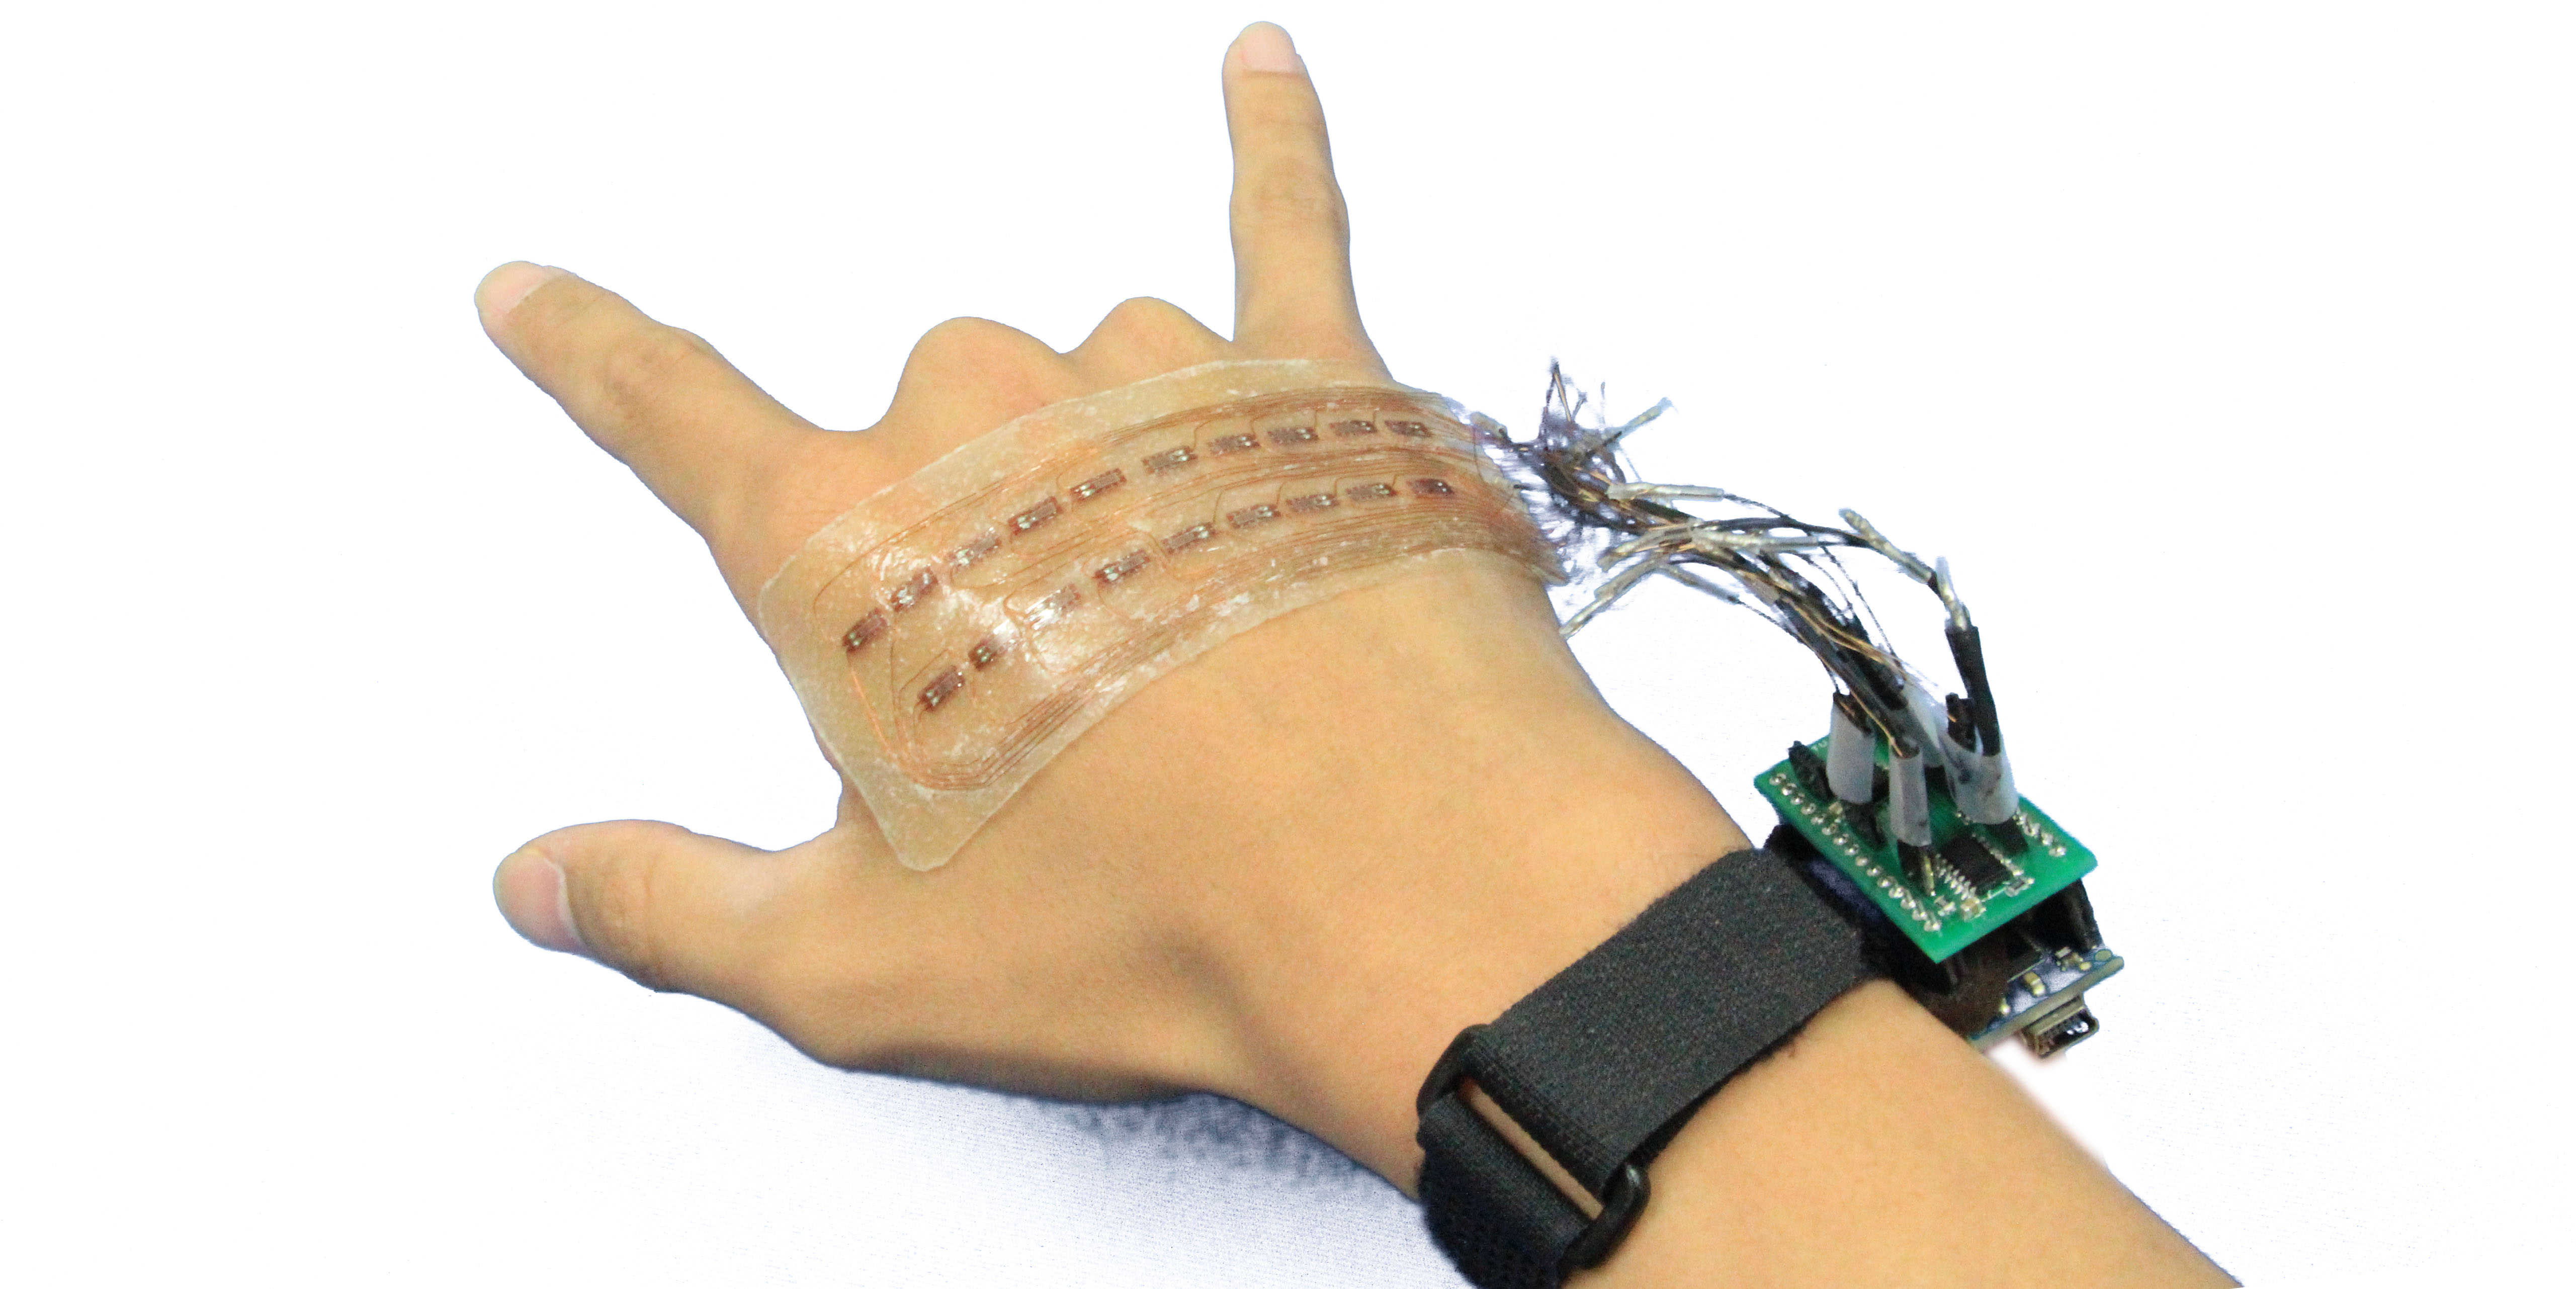
\includegraphics[width=1\columnwidth]{figures/BackHand.jpg}
  \caption{\getTitleName\ is a prototype that senses physical properties on the back of hand for hand gesture detection.}
  \label{fig:FIGURE1}
  \end{center}
\end{figure}

The second classification is the measurement of physical properties from the wrist. Capacitive sensing \cite{Rekimoto:2001:GGU:580581.856565}, force sensing approaches \cite{Dementyev:2014:WLG:2642918.2647396}, and vision \cite{Fukui:2011:HSC:2030112.2030154} have been used to sense changes in the physical properties of the wrist. Because of the reduced movement of the tendons compared to finger sensing, these approaches provide significantly lower accuracy even with a small number of gestures (2, 5, and 8 gestures respectively).

\begin{figure}[b]
  \begin{center}
  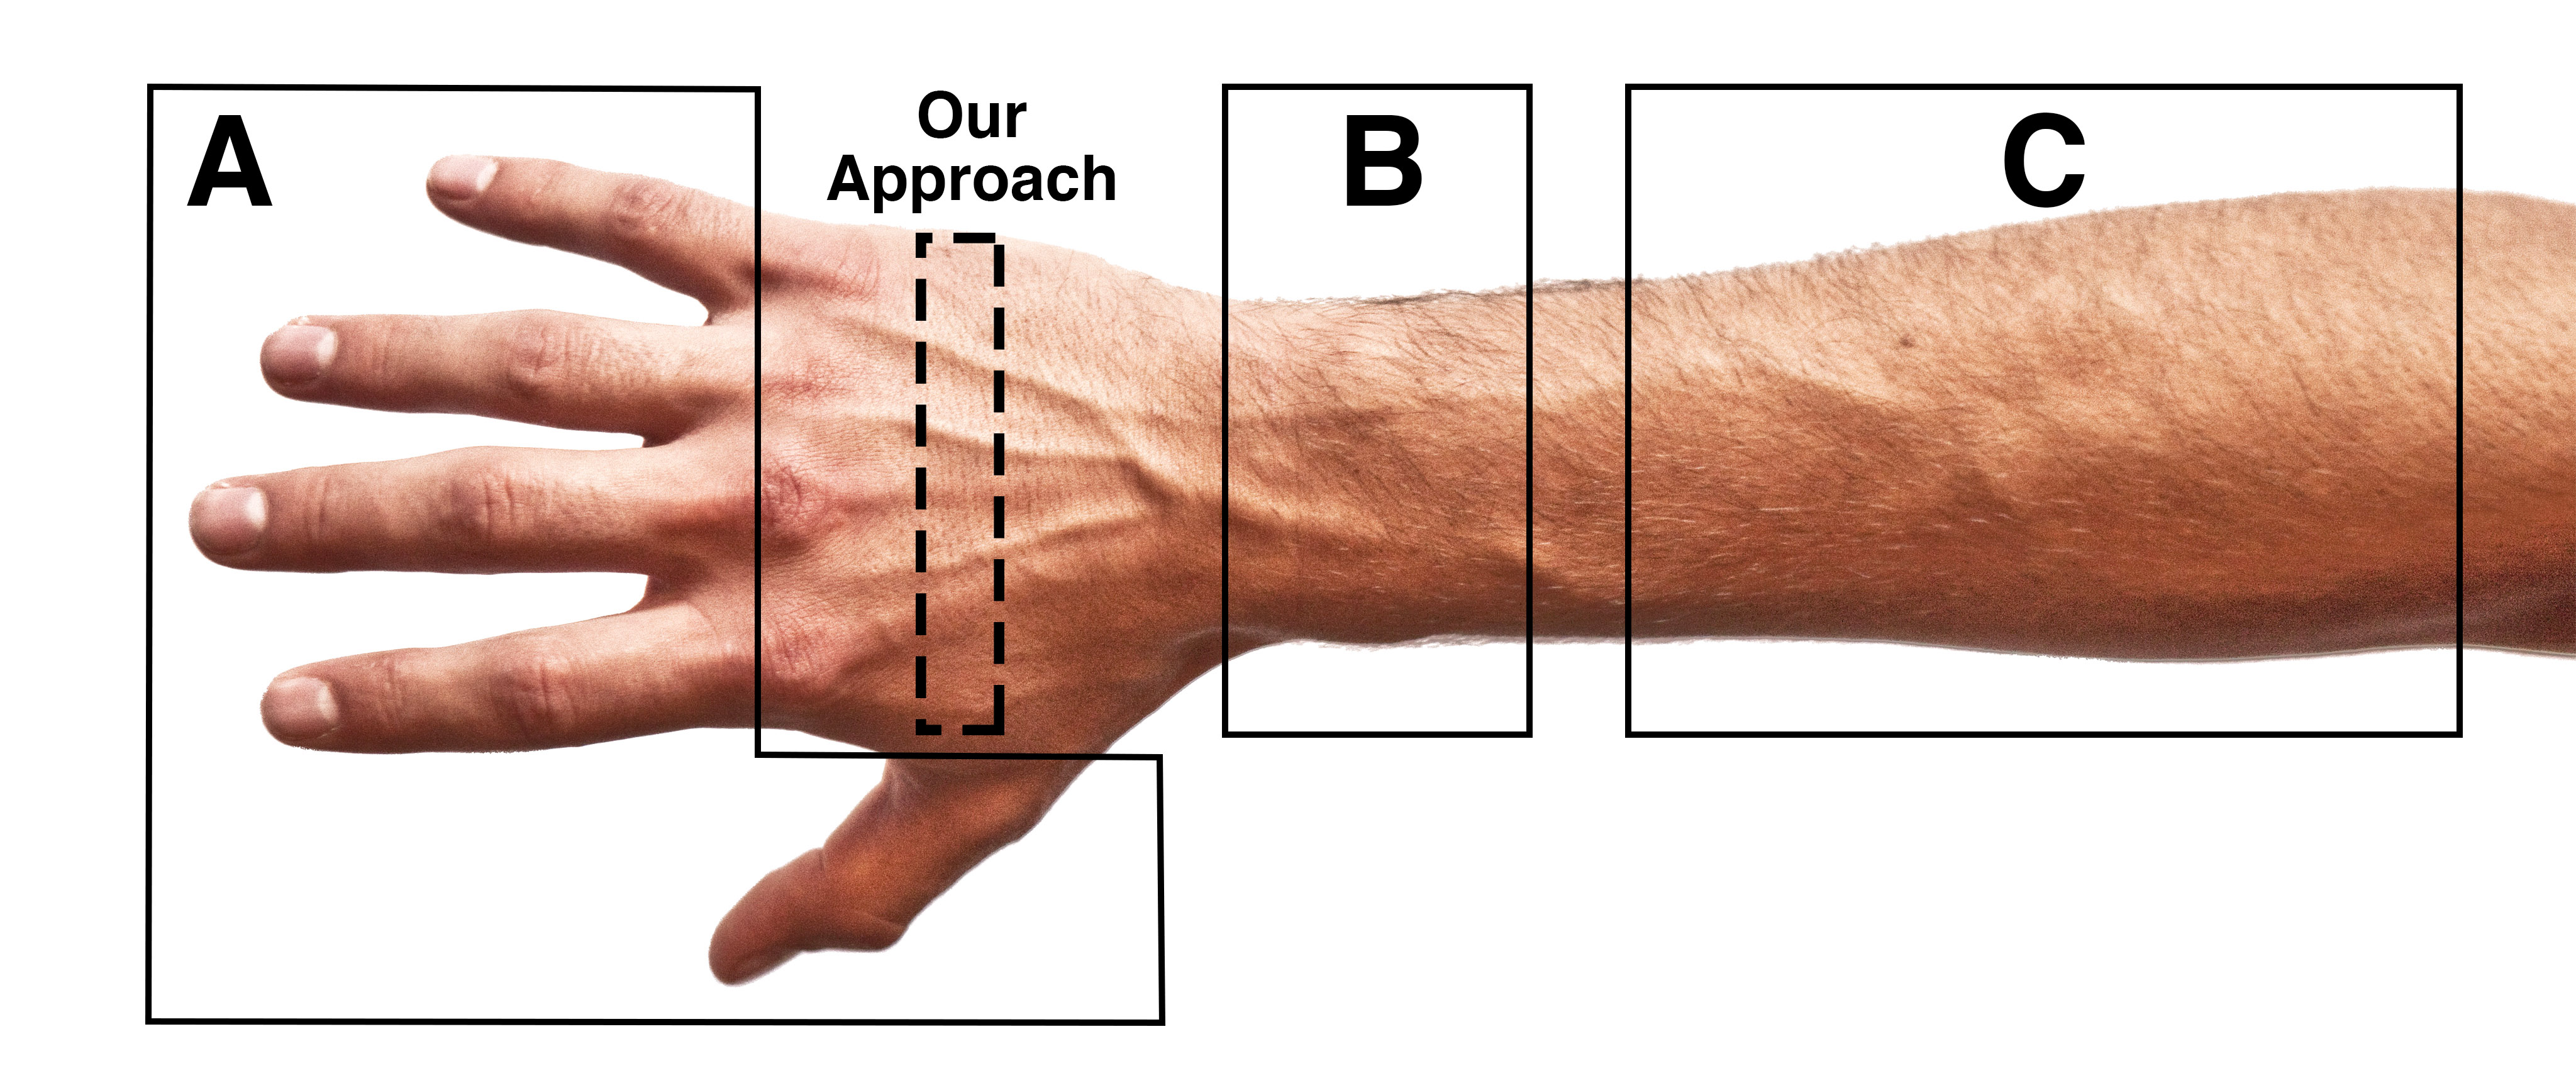
\includegraphics[width=1\columnwidth]{figures/HandTarget.jpg}
  \caption{The three common body parts as sources of a sensor's input signal for a hand gesture interface include (A) the fingers, (B) the wrist, and (C) the arm.}
  \label{fig:HandTarget}
  \end{center}
\end{figure}

The third classification uses forearm sensing to extract movements and gestures of a user's finger. Arm-based sensing measures electromyography (EMG) caused by hand gestures \cite{Myo, Saponas:2009:EAI:1622176.1622208}. It senses full hand movements (eg. clenched fist and splayed fingers) better than finer gestures such as moving a single finger.

Although the old colloquialism ``like the back of your hand'' suggests, we are not necessarily familiar with our own bodies. As shown in \autoref{fig:HandTarget}, the back of the hand is closer to fingers, and the movement of tendons can be observed and sensed more clearly than at the wrists and forearm. Sensors placed at this location also do not interfere with finger movement nor reduce the sense of touch compared to glove-based approaches. In this work, we explore sensing the back of hands for hand gesture detection.

Our prototype, \getTitleName\ (\autoref{fig:FIGURE1}), uses a total of 19 strain sensors in a 2-row configuration to measure the physical changes on the back of hands at a sampling rate of 75 Hz. A customized Arduino Nano shield circuit board is built for sensor signal conditioning. To better understand the areas that provide better gestural recognition accuracy, we conducted a user study to collect data by affixing our prototype to 8 specified rows evenly spaced from the metacarpophalangeal joints (MCP, the knuckles between the hand and fingers) to the head of ulna (tip of the wrist) while performing a number of 16 gestures. From the results of machine learning, the most promising location on the back of hand is found on the second and third row from the MCP joints. While an gestural recognition accuracy rate of 27.4\% is low in a leave-one-user-out cross validation, the accuracy rate is 95.8\% in a 10-fold cross validation. A visualization shown as heat maps assists our understanding towards the difference of sensor reading patterns among individuals and among various gestures.

Contributions of this paper are:
\begin{itemize}
\item We explored a new signal source, tendon activities on the back of hand, for hand gesture recognition.
\item We developed a prototype using strain sensors that can sense a large variety of gestures per user at higher accuracy than wrist-based approaches. 
\item We identified the most promising location in row configuration on the back of hand to be near the metacarpophalangeal (MCP) joints.

\end{itemize}


\section{RELATED WORK}

The growing number of a new interaction modality: body-worn hand gesture interfaces which senses the human-hand gestures as a wearable platform has led to attempts in categorization of those. One of the taxonomies of body-worn hand gesture interfaces is based on the source of the sensor's input signal which can be classified into three categories.

\subsection{Finger-based Hand Gesture Interfaces}
To gather high accuracy information of hand movements, a common technique is to measure the overall flexion of the fingers. One approach is to instrument the hand with a data glove-like hand gesture interface \cite{4539650, 1546364, 806717, tsukada2001ubi} which is equipped with a number of sensors that capture physical data about hand position, orientation, and bending angles of fingers.
For instance, the CyberGlove \cite{1414484} is currently considered one of the most accurate glove systems for 3D modeling, robot control, and so forth \cite{Burdea:2003:VRT:829566, LaViola:1999:SHP:864649}, and the 5DT Glove \cite{5DT} is famous in virtual reality. 
Although most of these finger-based systems provide high accuracy in measuring the degrees-of-freedom (DoF) of human hands, they suffered from several drawbacks. 
Major limitations originated from the cloth support and the mechanical structure \cite{4539650}
, which acted as a constraint on the user’s hand. For example, they have to be worn on the fingers to measure the flexion of the fingers. Such complications may not only reduce dexterity of the hand but blunt tactile sensitivity. Additionally, these systems can be complex, expensive, and cumbersome for users.

To overcome the discomfort of data glove, another approach uses wearable cameras to recognize finger gesture. Vision-based systems can be worn on some parts of the body such as Digits \cite{Kim:2012:DFI:2380116.2380139} and another system \cite{6855631} which are wrist-worn sensors based on 3D infrared camera and time-of-flight (TOF) camera respectively, SixSense\cite{Mistry:2009:SWG:1667146.1667160} which senses colored markers on the fingertips through wearing a lanyard necklace with a camera. By recovering 3D articulated hand poses, they provide high-fidelity sensing without wearing the glove. However, because of the fundamental limitation of cameras, the visible occlusion resulting from crossing finger, a significant elevation from the wrist, heavy computation requirement of 3D reconstruction technology, large power consumption and expensive cost are problematic for these vision-based systems.

\subsection{Wrist-based Hand Gesture Interfaces}

From another approach, a number of lightweight systems measuring physical properties from the wrist to detect gestures have been proposed. 
Although wrist-based hand gesture interfaces are much rare compared to finger-based hand gesture interfaces, they are the most friendly and acceptable interfaces due to their placement.

Instead of providing high-accuracy sensing, GestureWrist \cite{Rekimoto:2001:GGU:580581.856565} uses capacitive sensors to recognize a small set of gestures. WristFlex \cite{Dementyev:2014:WLG:2642918.2647396} uses an array of force sensitive resistors (FSRs) supporting 5 gestures at an accuracy rate greater than 80\%. Another system \cite{Fukui:2011:HSC:2030112.2030154} places infrared transmitters and receivers around the wrist to recognize hand gestures. Hambone \cite{4373768} employs bio-acoustic method performing hand motions through the wristband enhanced with piezoelectric sensors, supporting classification accuracies around 90\% for 4 gestures. While all these devices overcome some of the limitations of the data glove-like systems (e.g., most have no cloth), they appear to be unsuitable for applications that require high accuracy measurement and the diversity of gesture types. 

\subsection{Arm-based Hand Gesture Interfaces}

Arm-based hand gesture interface is another approach to explore hands-free and implement-free input techniques. Some research projects based on muscle-computer interface \cite{Saponas:2009:EAI:1622176.1622208} use forearm electromyography to decode the signal from motor neurons associated with muscle activation and recognize four-finger pinch gestures at an accuracy rate of 79\%. A commercial product named Myo \cite{Myo} also uses EMG for gesture detection. However, finer gestures involving single finger movements are not discernible to such devices. In addition, compared to the aforementioned interfaces, EMG systems require high data rate and have high power consumption due to extensive signal processing. 

As mentioned above, these interfaces with a variety of sensing technologies in different places to assess finger movement are the most common approaches to recognize hand gestures. However, \getTitleName\ senses hand gestures by exploring the back of hand which is not in the three classifications. We achieved 95.8\% average accuracy for 16 popular hand gestures when personalized for each participant. Additionally, we are not aware of any research that explored the back of hand to recognize hand gestures.

\begin{figure}[b]
 \begin{center}
  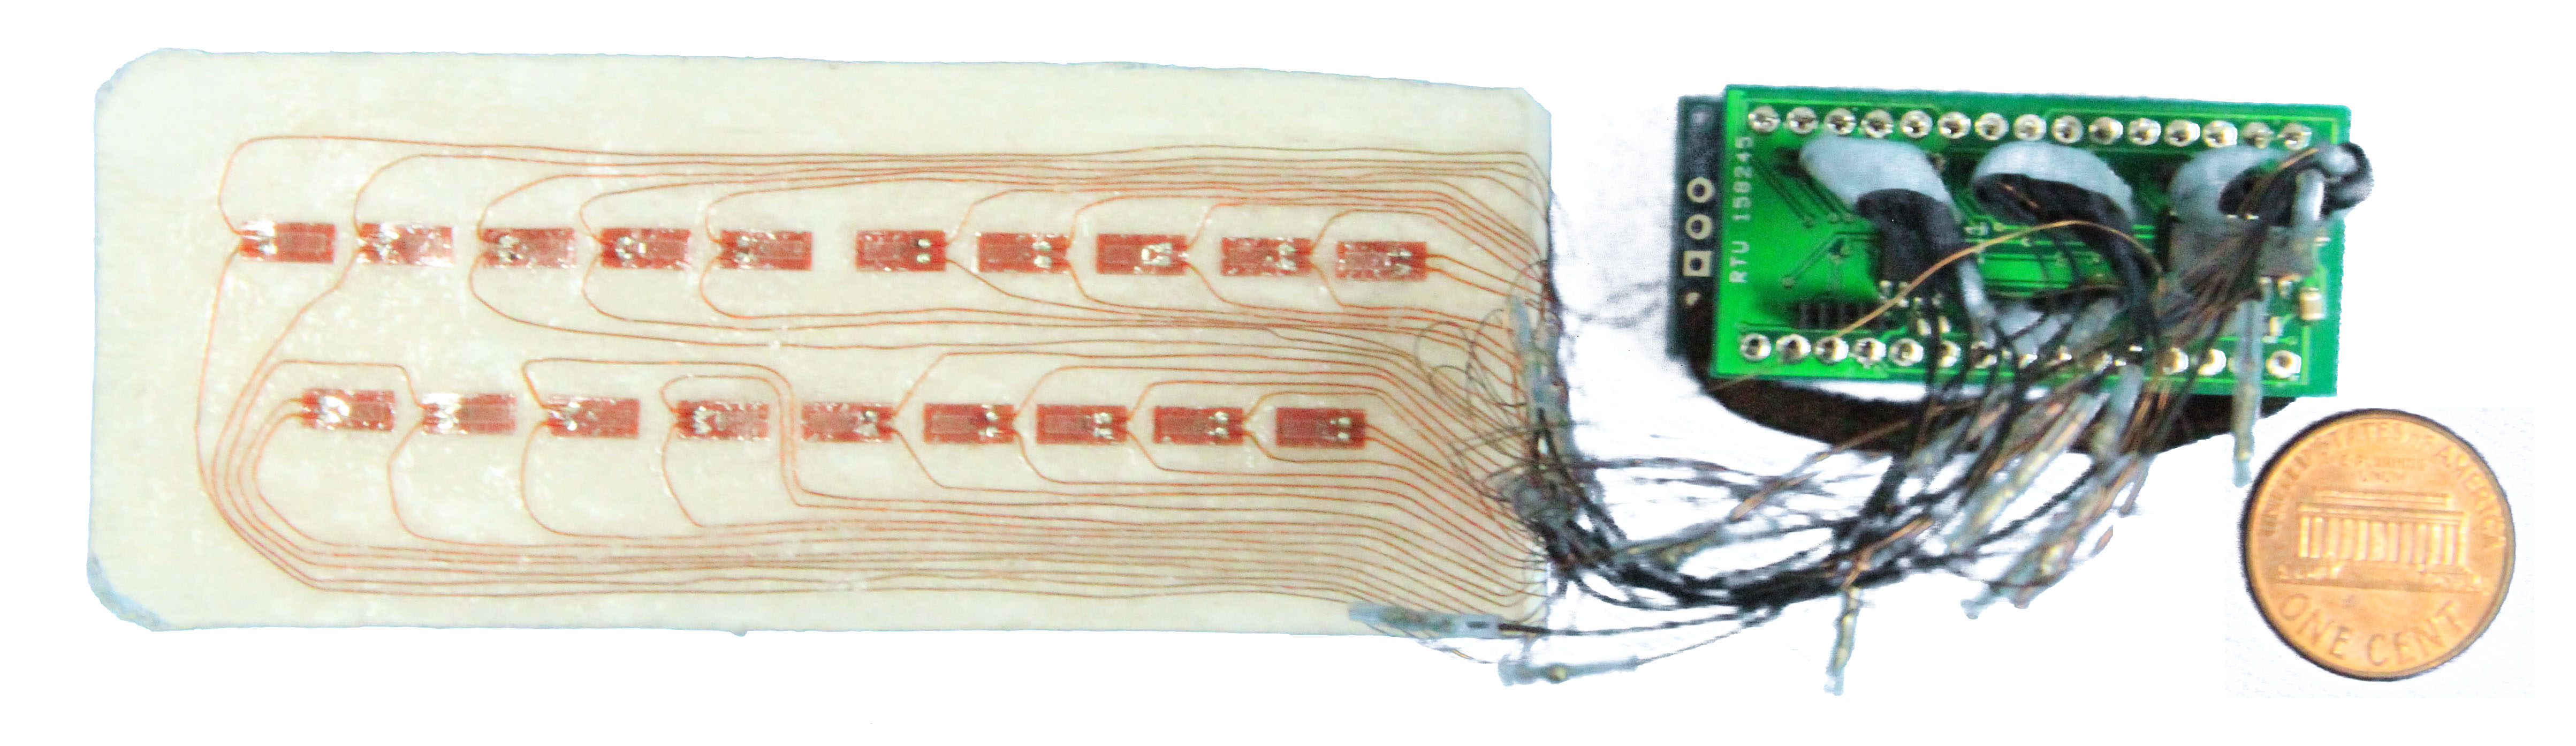
\includegraphics[width=1\columnwidth]{figures/prototypeV2.jpg}
  \caption{The layout shows a total of 19 sensors with a base length of 6.3 mm distributed into a 2-row configuration on an artificial skin. The strain sensors should avoid physical contact with each other by leaving a spaced interval of 2 mm between the neighboring sensors in a row. Therefore, a number of 10 sensors fits the hand width of a normal person. The second row includes 9 sensors to increase resolution and to measure the physical properties along the vertical direction between each spaced interval of the first row.}
  \label{fig:tie}
  \end{center}
\end{figure}

\section{BACKHAND-PROTOTYPE DESIGN}

Physical changes on the back of hand caused by finger motions and gestures are visible to the human eye. However, there is still difficulty on detecting it through most sensing techniques because such physical changes are very small in comparison to that of finger joint movements. Moreover, physical changes on the back of hand varies from person to person. Accordingly, we have two major requirements. First, a small and light device must be able to sense small physical changes. Second, a device must be able to extract individual information from multiple spots on the back of a human hand. Among a variety of sensing techniques, we conclude that strain gauge sensors best fit our requirements for this prototype.
 
\subsection{Hardware} 

Strain gauge sensors are sensitive devices used to measure very small strain and elongation of an object such as buildings, foundations, and other structures. In order to accomplish such measurement, a strain gauge must be adhesively attached to the object. Any tension or compression on the object leads to changes in the electrical resistance of the sensor.

\begin{figure}[t]
  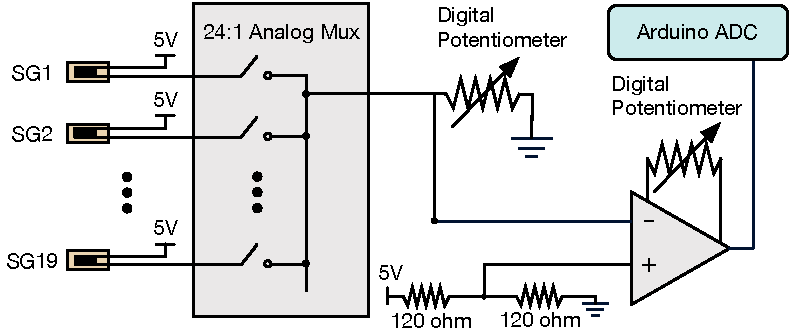
\includegraphics[width=1\columnwidth]{figures/CompleteDiagram_v3.pdf}
  \caption{The complete circuit diagram. Note that SG stands for strain gauge. The 24:1 analog multiplexer is practically made up of 3 analog multiplexers.}
  \label{fig:completeCircuitDiagram}
\end{figure}

In our prototype, the sensing stage of our prototype consists of a reusable hydrogel-based artificial skin and 19 120-ohm 2-mm strain gauge sensors. The artificial skin is attached to the back of hand and acts as a sensor carrier. As shown in \autoref{fig:tie}, the sensors are distributed into a 2-row configuration. The following sentences explain for such sensor layout. An average of human hand width is approximately 81 mm \cite{Kulaksiz2002257}, and the base length of a 2-mm strain gauge is 6.3 mm. In order to avoid physical contact between any two neighboring sensors in a row causing strain interference, a spaced interval of 2 mm separates them, resulting in 10 strain gauges in a row across the hand width. Without the loss of strain measurement along the vertical direction between the two neighboring sensors, a second row with 9 sensors, each of which is vertically aligned with each center of the spaced intervals on the first row, is placed under the first row. The sensor array measures the deformations of multiple individual spots of the artificial skin caused by physical changes on the back of hand. Thus, our prototype is made possible to become a hand gesture interface for general users.

\begin{figure}[b]
  \begin{center}
  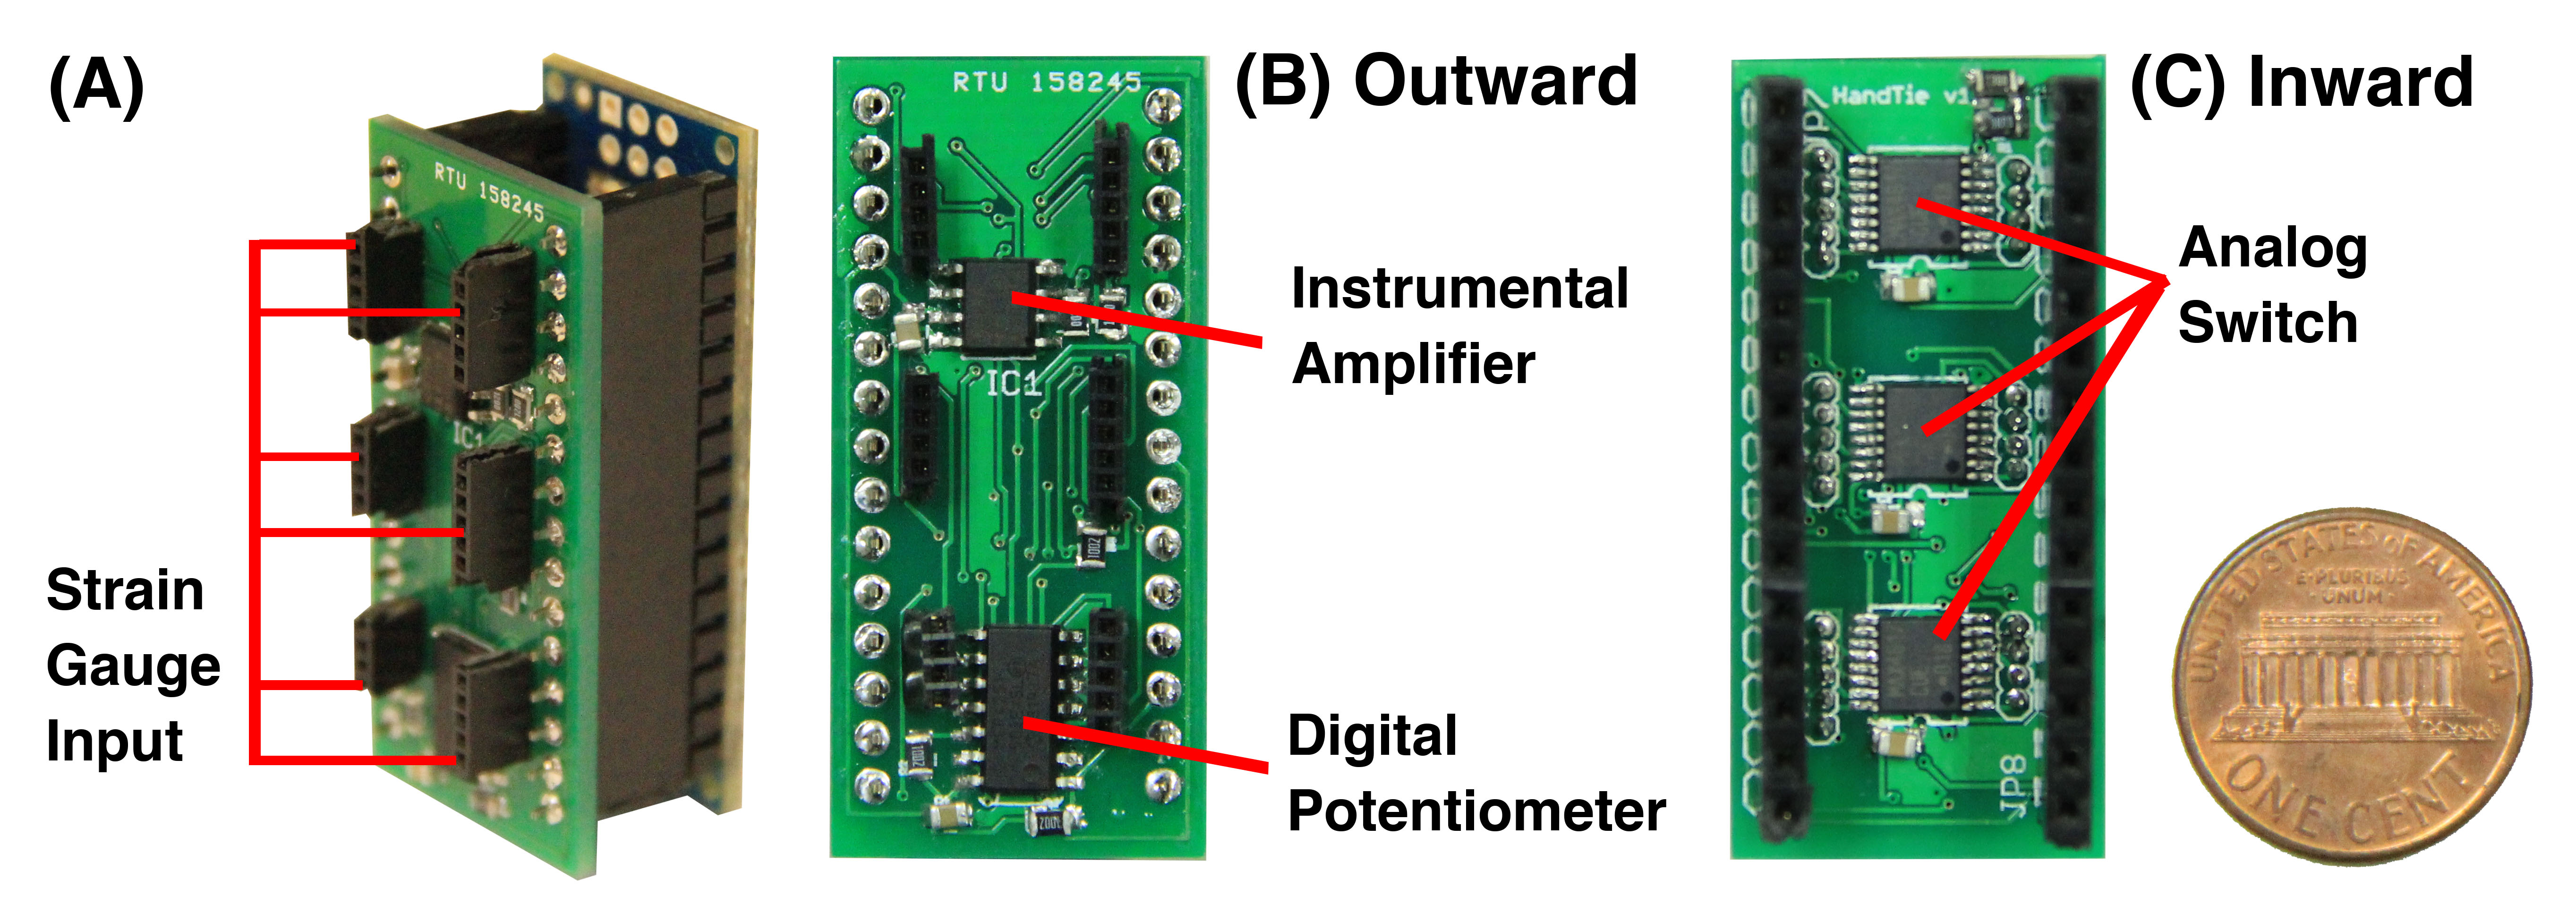
\includegraphics[width=1\columnwidth]{figures/harwareV2.jpg}
  \caption{ A customized 2-layer Arduino Nano shield circuit board used for signal conditioning is shown in (A) whose outward side is shown in (B) and inward side is shown in (C).}
  \label{fig:hardware}
  \end{center}
\end{figure}

Next, the signal conditioning stage includes a Wheatstone bridge, 3 8-to-1 analog switches (MAX4617, Maxim Integrated), a dual digital potentiometer (MCP4251, Microchip), and an instrumental amplifier (AD623, Analog Devices). Finally, the processing stage includes an Arduino Nano used to sample the sensors and control chips in the signal conditioning stage. The complete circuit diagram is shown in \autoref{fig:completeCircuitDiagram} and a customized circuit board is shown in \autoref{fig:hardware}.

The 19 sensors are read sequentially through the analog switches, so each sensor is electrically connected at a time. Once a sensor is active, the sensor became one of the 4 resistors on the Wheatstone bridge. Since the resistance of each sensor varies under no applied external force, a digital potentiometer in series with the connected sensor is used for calibration. Another digital potentiometer serves the purpose of amplifier gain adjustment. In our prototype, the instrumental amplifier gain is set to be approximately 800 to 1000. Due to the dynamic response time of the amplifier, a 100-microsecond delay is added between each reading leading to a sampling rate of 75 Hz for our prototype.


\subsection{Machine Learning}
A support vector machine (SVM) is a novel supervised learning method that basically analyses the given data and recognizes patterns from it.
We used LIBSVM tool \cite{CC01a}, an open source library for SVM. 
We scale each feature to the range of 0 to 1 and then train a multi-class SVM classifier with a Radial Basis Function (RBF) kernel.


\section{EVALUATION: MOST PROMISING LOCATION}

The purpose of this evaluation is to investigate the accuracy of several row configurations ranging from back of the hand to wrist, and to uncover the most promising location that maximizes the performance of identifying hand gestures. 

Based on our observation and assumption of the anatomy of finger tendon networks, a row configuration laying across the hand width is the most intuitive pattern to capture all tendon and muscle activities caused by movements of each finger. Although it is reasonable that the highest accuracy rate (e.g. \textgreater90\%) may occur by covering the entire hand full of sensors, reaching high accuracy rate with less coverage area is worthy of being studied.

In addition, we provide the accuracy rates of each row configuration and visualizations of physical changes on the back of hand caused by gestures that are collected from all participants. These can enable us to understand, illustrate, and provide insights into the physical properties of the back of hand. %by collecting data

\subsection{Study Design}
We recruited 10 participants (4 females, 9 right-handed) aged between 20 and 32 (mean: 23.2) to test 16 gestures, shown in \autoref{fig:gestureSet16}.

\begin{figure}[b]
  \begin{center}
  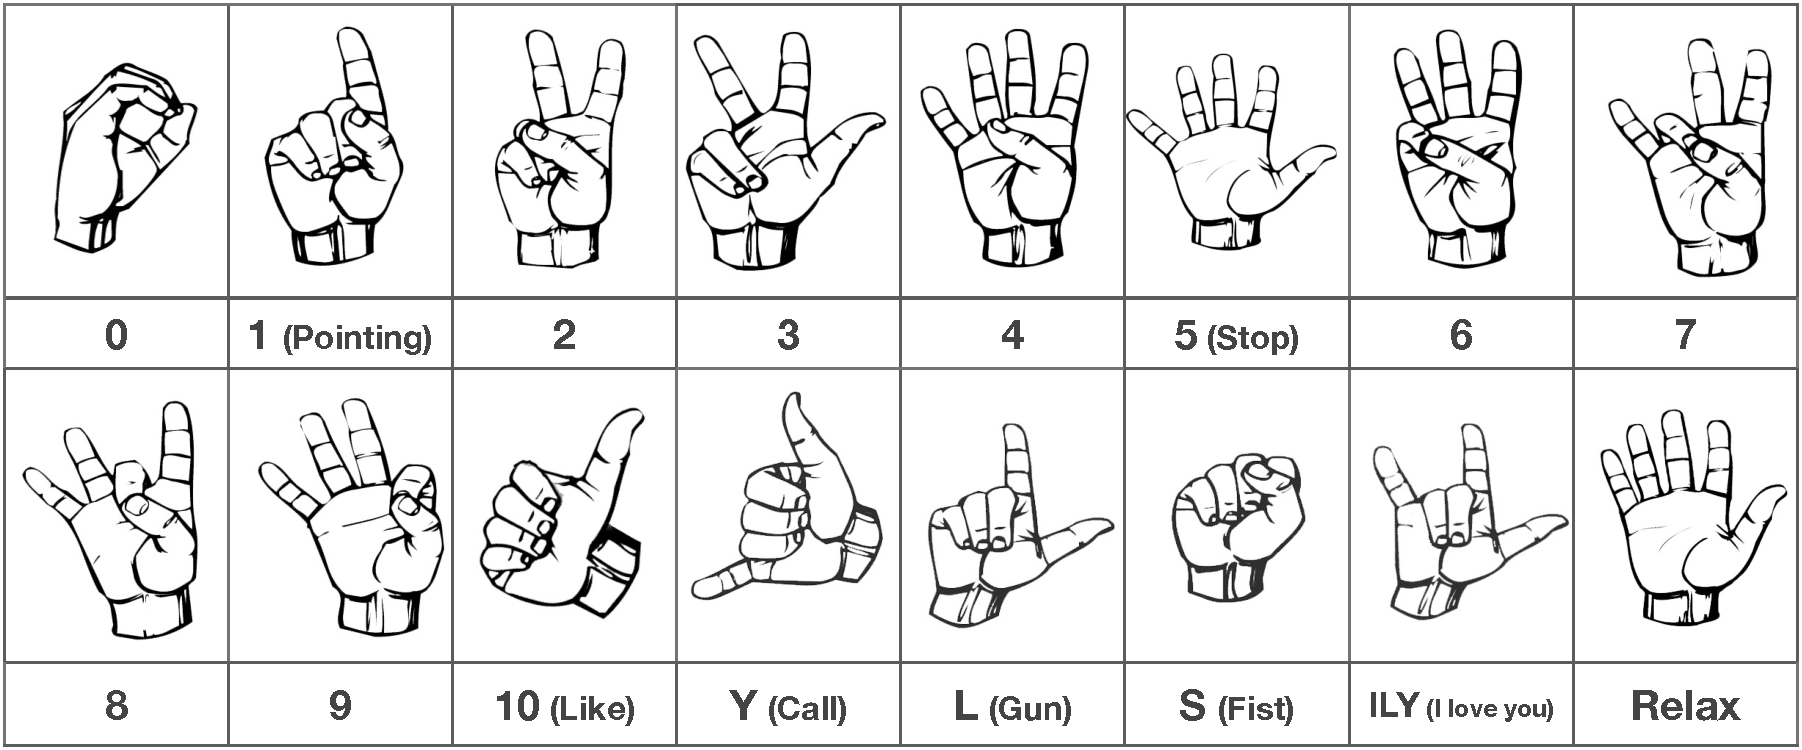
\includegraphics[width=1\columnwidth]{figures/gestureSet_16_v3.pdf}
  \caption{16 gestures were chosen from American Sign Language and popular Asian gestures.}
  \label{fig:gestureSet16}
  \end{center}
\end{figure}

\subsubsection{Gesture Set}
We mainly picked a gesture set from American Sign Language (ASL) such as digits from 0 to 10. In addition to the ASL gestures, we chose 4 gestures possessing significant cultural meanings in Asia such as digit ``six'', ``seven'', and ``zero'', and ``I-love-you'', each of which also coincides with ``Y'', ``L'', ``S'', and ``ILY'', respectively, in ASL. Therefore, the gestures in \autoref{fig:gestureSet16}\ are denoted using ASL letters. Finally, a neutral hand posture, relaxed gesture, along with 15 gestures adds up to a total of 16 gestures.

\subsubsection{Procedure}
%see figure
\autoref{fig:StudyEnv}\ shows the study setup. The participants rested their right arm and wrist on the tilt platform and were seated on a chair whose height they could adjust to perform the tasks with ease. The monitor in front of the participants displayed instructions during the study.

%need to explain why 8 rows!!
Initially, 8 rows (16 positions) across participants’ back of the hand were uniformly sampled and marked. The sampling scope ranged from the position of metacarpophalangeal joints (MCP, the knuckle between the hand and the finger) to the head of ulna (at the wrist).%see figure 
 The markers served as affixing targets for artificial skin composed of arrays of 19 strain gauges are shown in \autoref{fig:studyProcedure}.

\begin{figure}[t]
  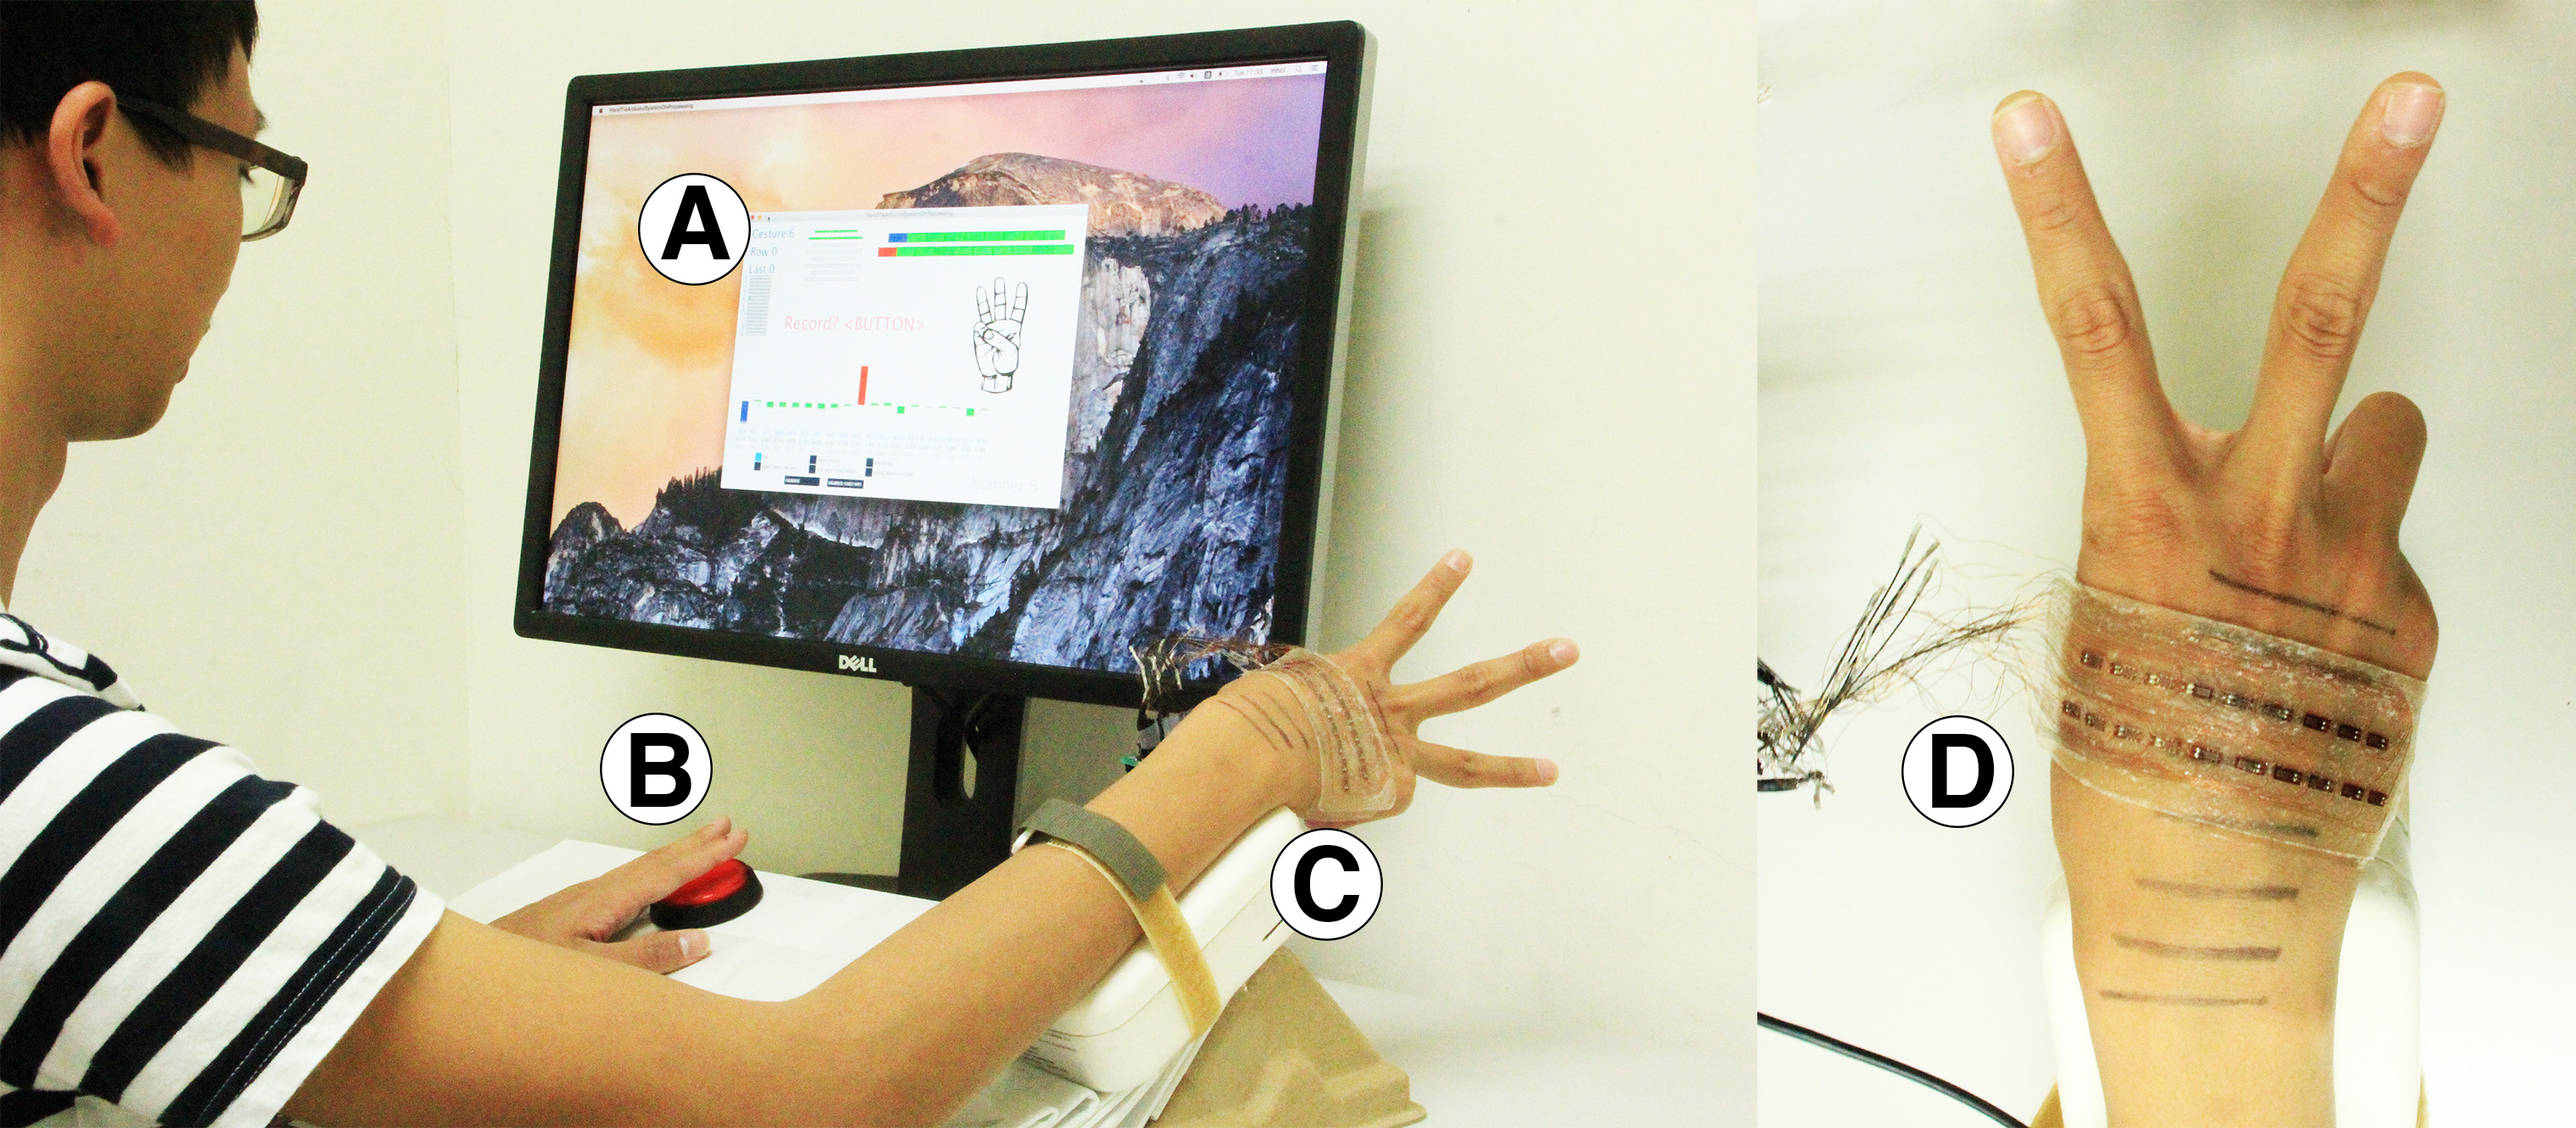
\includegraphics[width=1\columnwidth]{figures/StudyEnv.jpg}
  \caption{Study Setup:
            (A) monitor for on-screen instruction.
            (B) A button pushed by a participant to begin recording sensor readings while performing a gesture from the on-screen instruction.
            (C) A tilt platform for the arm to rest on.
            (D) Our prototype attached to the back of hand at specified locations. }
  \label{fig:StudyEnv}
\end{figure}

\begin{figure}
  \begin{center}
  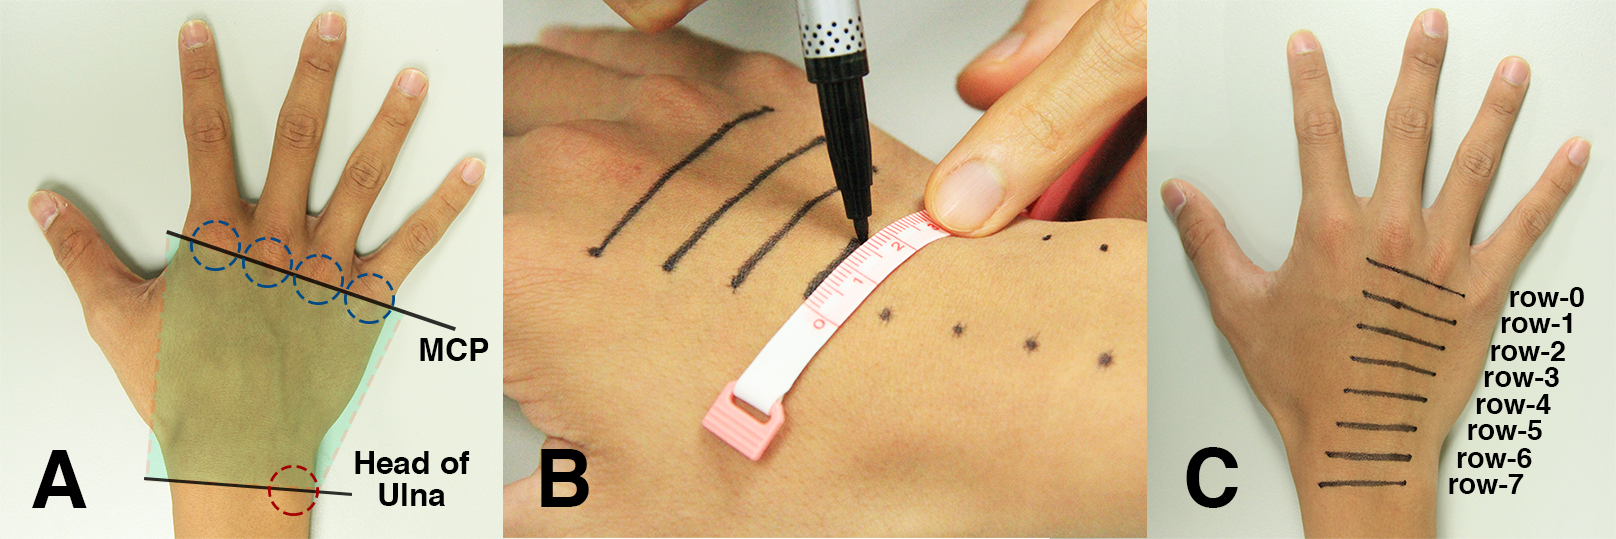
\includegraphics[width=1\columnwidth]{figures/studyProcedure.jpg}
  \caption{The procedures of marking the 8 rows on the back of hand.
          (A) Locate the MCP joint positions and the head of ulna. 
          (B) Evenly mark 8 points from the index MCP joint to the imaginary horizontal line that goes through the head of ulna. Evenly mark another 8 points from the pinky MCP joint to the head of ulna. Draw 8 lines on the back of hand.
        %   (B) Divide the length between an MCP joint and the imaginary horizontal line going through the head of ulna by 8. 
          (C) 8 rows evenly spaced between the MCP joint and the head of ulna are marked where our prototype aligns.
  }
  \label{fig:studyProcedure}
  \end{center}
\end{figure}

We then affixed the artificial skin composed of arrays of strain gauges to these 8-row markers on the right hand for 4 rounds (2 rows each time). At each round, each participant performed each of 16 gestures from on-screen instructions. Each gesture was collected 10 times. Each of them was sampled at 10 Hz in a duration of 2 seconds.
The order of the gestures was randomly selected. 
Overall, the study took approximately 80 minutes per participants.

\vspace{10mm}

\begin{figure*}[t]
 \begin{center}
  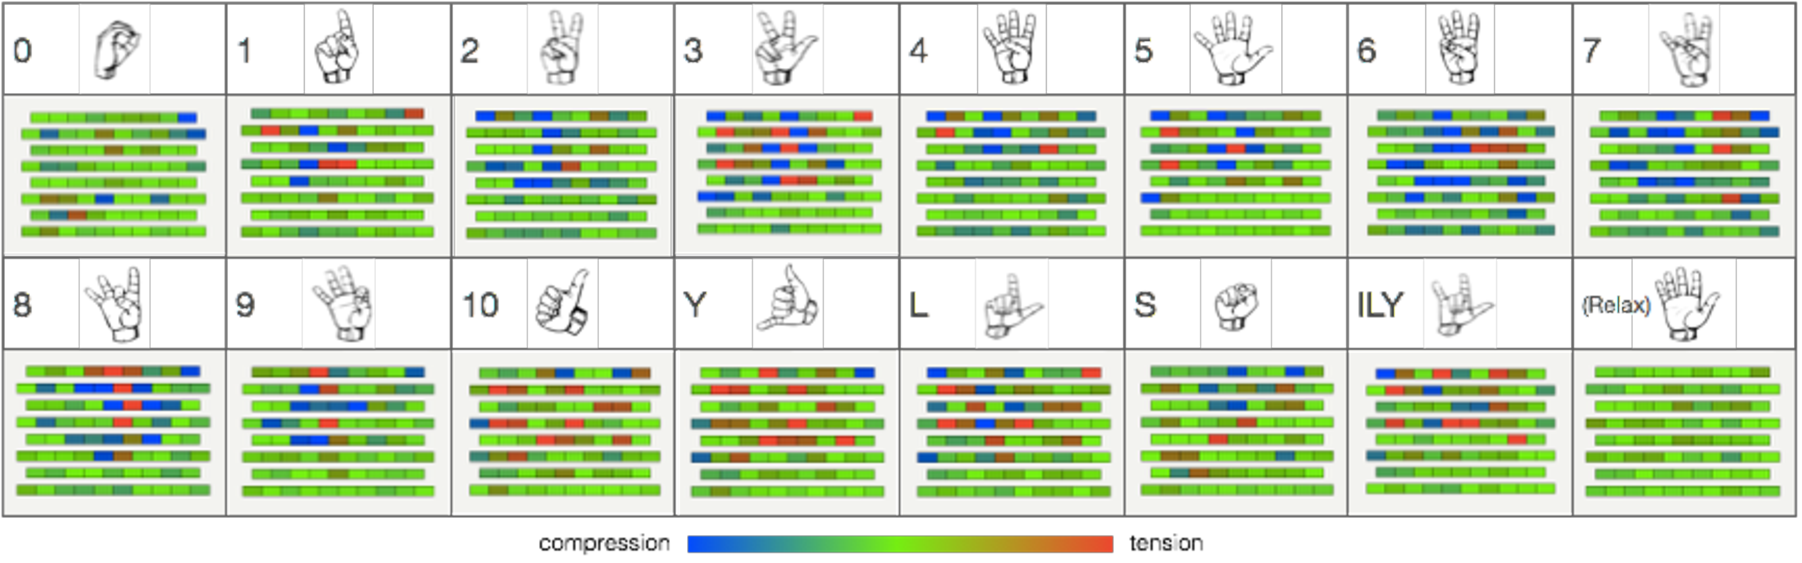
\includegraphics[width=2\columnwidth]{figures/user16GesturesSV_v3.pdf}
  \caption{ 16 heat maps display all 16 gestures performed by one of the participants. Each entry is an average heat map of 10 trials of a gesture. The sensor reading patterns are significantly different across 16 gestures.
  }
  \label{fig:user16GesturesSV}
  \end{center}
\end{figure*}

\subsection{Results}

Our results consist mainly three parts. The first part is a visualization of physical changes on the back of hand. The second part is a leave-one-user-out cross validation to test the feasibility of building a general model across participants. The last part is the determination of the most promising location through a personalized gestural recognition accuracy.

\begin{figure}[t]
 \begin{center}
  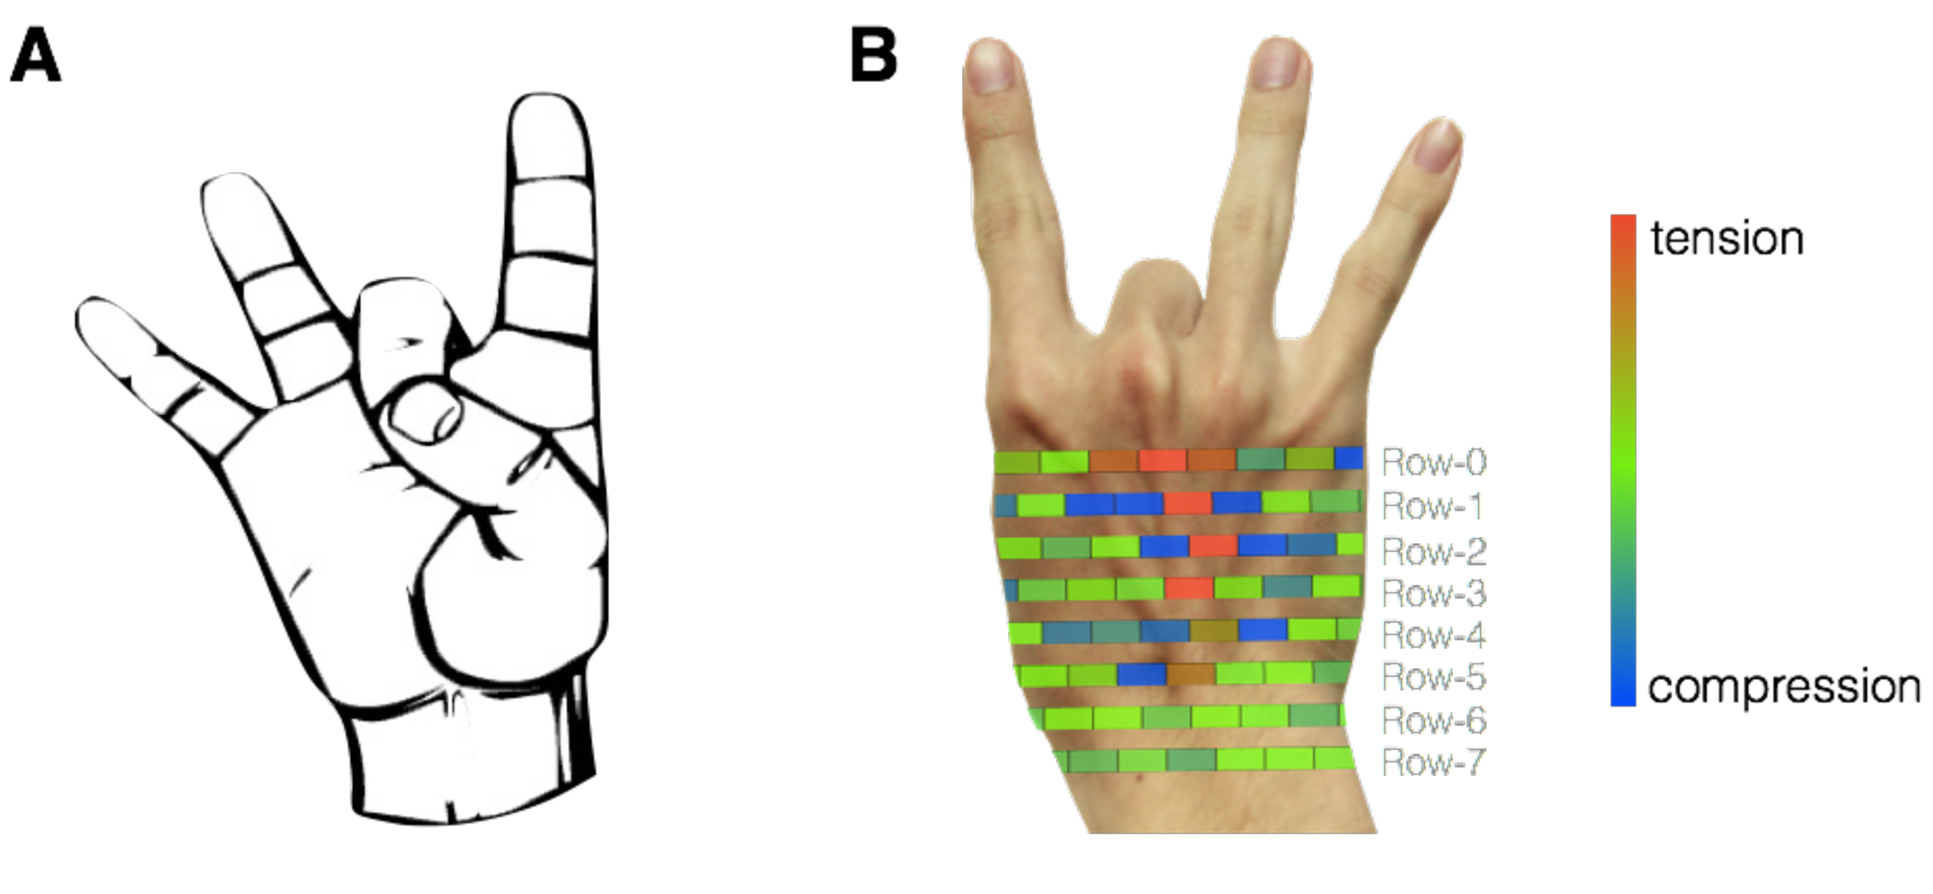
\includegraphics[width=0.9\columnwidth]{figures/Num8GestureV4.pdf}
  \caption{
    (A) A gesture of ``8'' from ASL is performed.
    (B) A heat map overlapped with a hand is illustrated to show the sensor values of each strain gauge resulting from the gesture of ``8'' performed by a user.
  }
  \label{fig:Num8Gesture}
  \end{center}
\end{figure}

\subsubsection{Heat Map Visualization}

The visualization is shown in heat maps which display a block with highest tension sensor value as red and highest compression value as blue. The color green represents the neutral state (without tension and compression) of a strain gauge. Other blocks with colors in-between the extremes of red and blue on the color spectrum feature sensor values between the highest tension value and highest compression value.

\begin{figure}[t]
 \begin{center}
  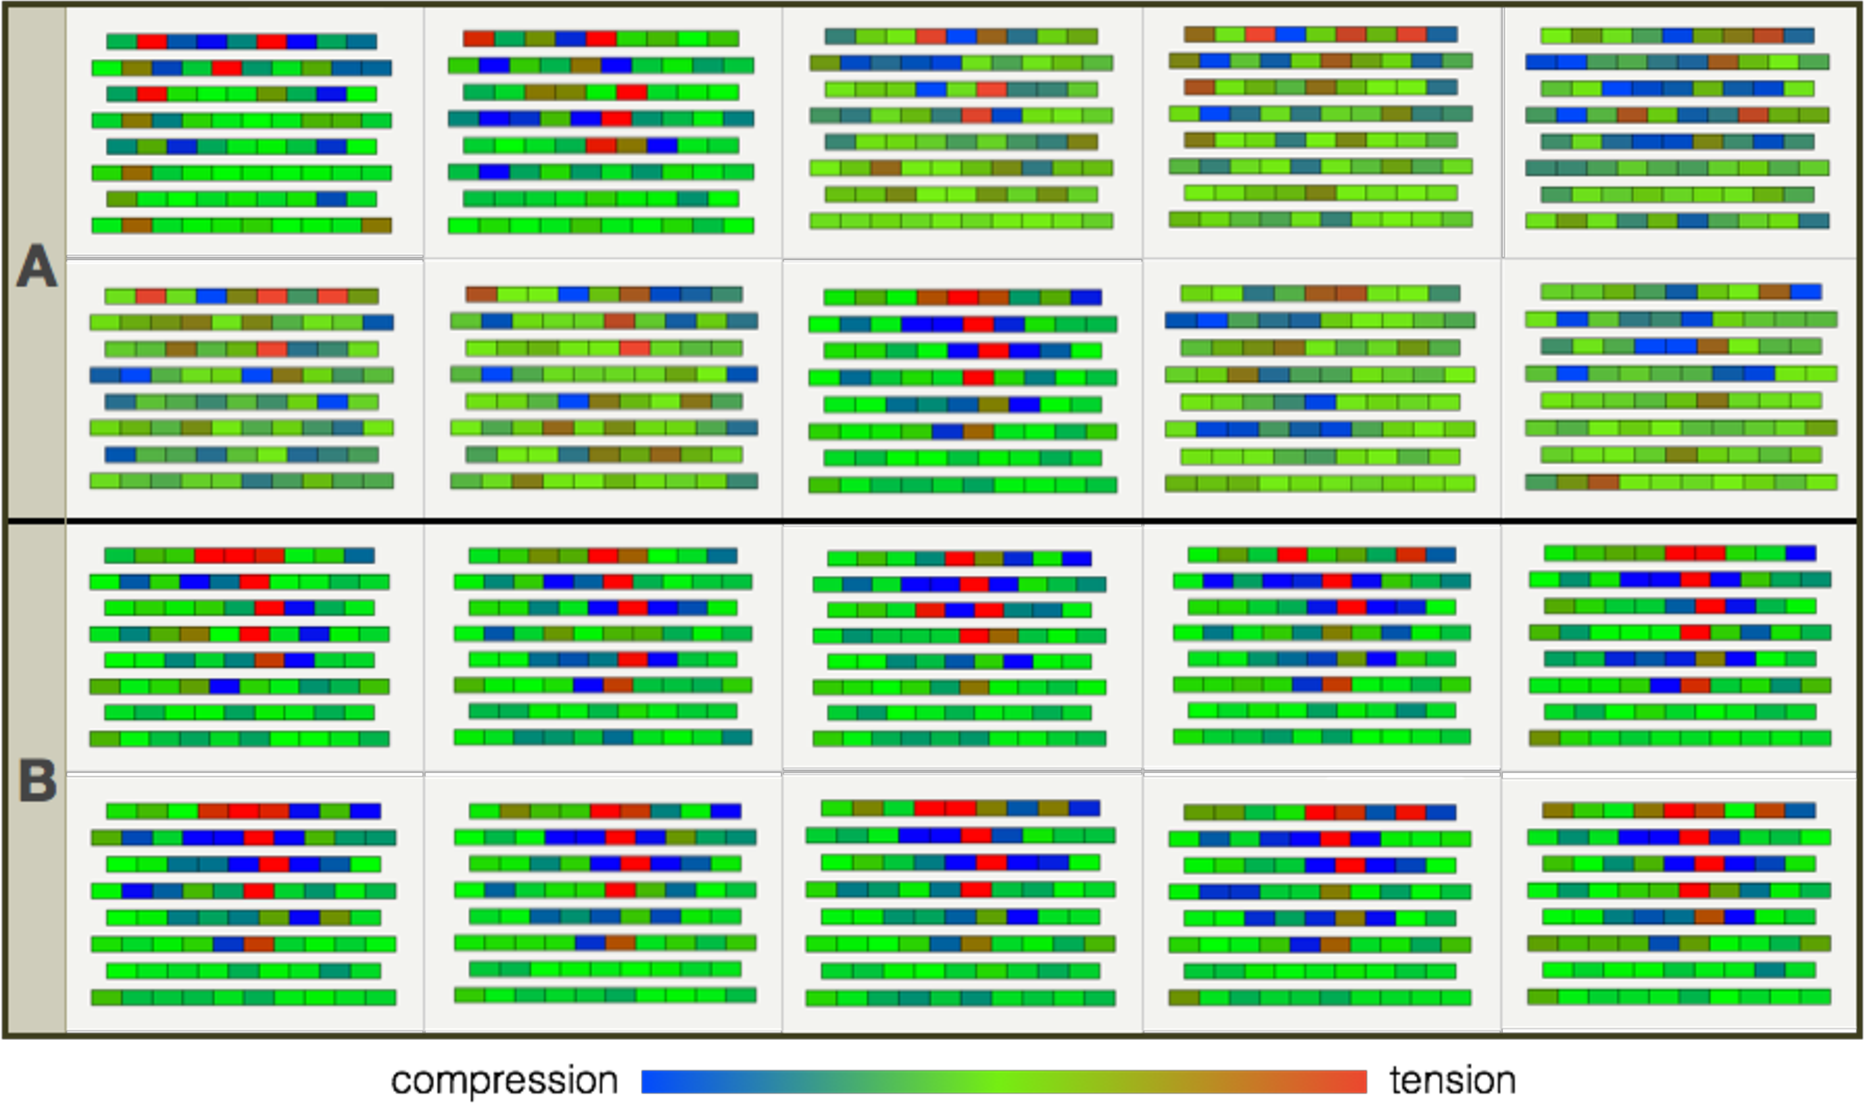
\includegraphics[width=1\columnwidth]{figures/SVisualNew_v3.pdf}
  \caption{
    (A) Each entry is an average heat map of 10 trials of gesture ``8'' performed by a single user. The color distributions of each heat map differ quite much from person to person.
    (B) 10 heat maps display all 10 trials of gesture ``8'' carried out by a participant. The color distributions remain fairly consistent throughout the trials.
  }
  \label{fig:SVisualNew}
  \end{center}
\end{figure}

\autoref{fig:user16GesturesSV}\ showing all 16 gestures performed by a participant implies that every pattern on the back of the hand has its unique gesture model inside it.
\autoref{fig:Num8Gesture}\ and \autoref{fig:SVisualNew}\ indicate heat maps of a gesture of ``8'' performed by participants.
From \autoref{fig:Num8Gesture}(B), the strain sensors attached along with the prominent, superficial tendon of middle finger are stretched, while sensors in-between tendons are compressed.
% The sensor reading patterns are significantly different across 10 participants in \autoref{fig:SVisualNew}(A) but consistent for a single user in \autoref{fig:SVisualNew}(B).
\autoref{fig:SVisualNew}(B) indicates the consistent reading patterns for a single user concluding the stability to utilize such signal source.
The sensor reading patterns are significantly different across 10 participants in \autoref{fig:SVisualNew}(A) implying the difference of both the prominence of tendons and the physical appearance of finger tendon networks among individuals.
% Based on the observations and results of the visualization, it is not difficult to find the reason why \getTitleName\ can be used to detect hand gesture due to each tendon activities on the back of hand while performing hand gesture.
The measurements of tendon activities contribute the visualization which leads to a better understanding of the back of hand that in turn possesses a potential for hand gesture recognition.

\subsubsection{Accuracy Rates}
We tested all 15 possible row configurations for determining minimum strain sensor coverage area on the back of hand including 8 single-row configurations (from row-0 to row-7) and all 7 two-adjacent row configurations (row-01, row-12, row-23, row-34, row-45, row-56, and row-67) of sensing locations from each participant.

\begin{figure*}[t]
 \begin{center}
  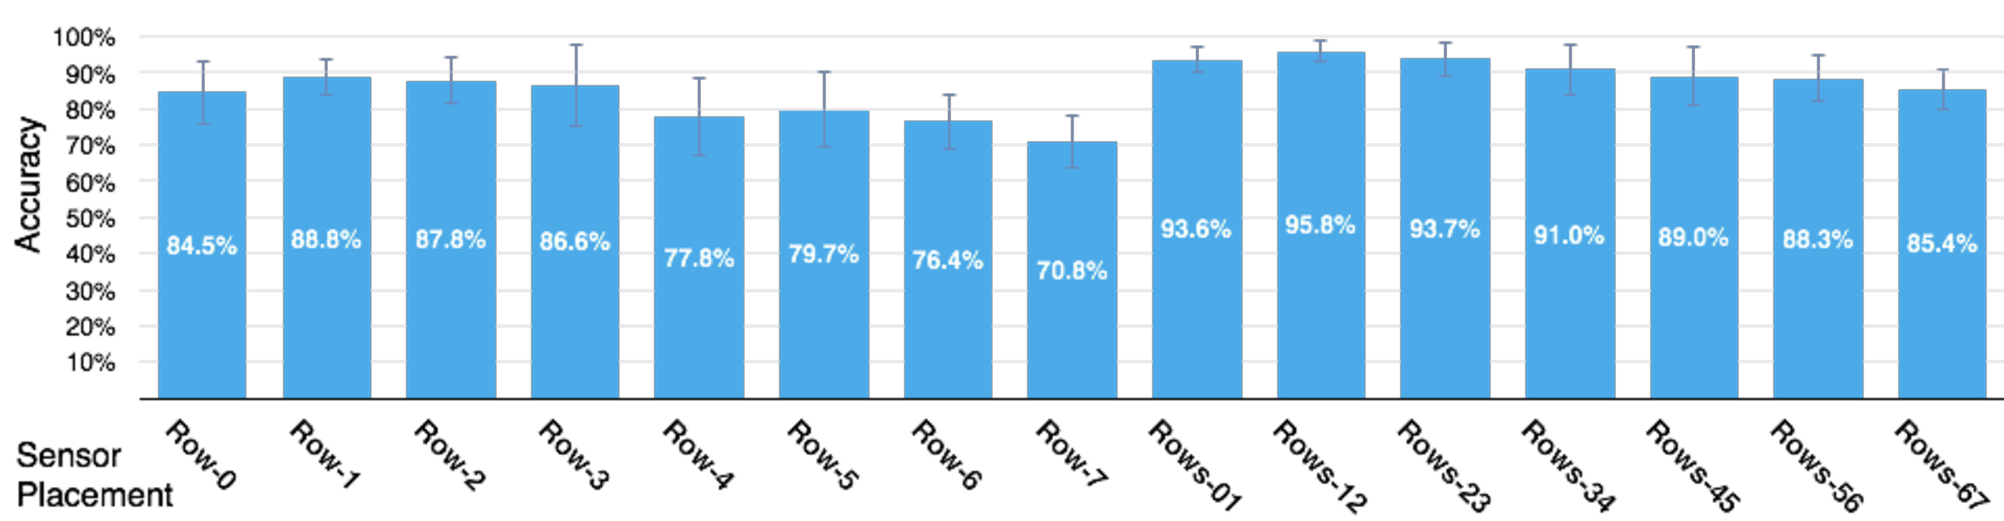
\includegraphics[width=2\columnwidth]{figures/10FCV_16_v3.pdf}
  \caption{
    The result of the average of 10-fold cross validations of all 10 participants. The value of each bar is an average of personalized accuracy rate in 10-fold cross validation of a row configuration across all participants.
  }
  \label{fig:accuracy16Gs}
  \end{center}
\end{figure*}

To understand how physical changes on the back of hand vary from person to person, the results of a leave-one-user-out cross validation are shown in \autoref{fig:LOO} where the value of each bar is an average of test results of each participant validated by the other 9 participants' training model of a row configuration on the back of the hand. The highest accuracy rate of 27.4\% occurs at the location of row-23. Hence, the low accuracy rates imply that physical patterns on the back of hand are likely to be in low similarity among individuals.

Based on the results from the leave-one-user-out cross validation, constructing a generalized model across general users is highly unlikely. Therefore, we delve into personalized accuracy rates and the aim for a most promising location.
% We tested all 15 possible row configurations for determining minimum strain sensor coverage area on the back of hand including 8 single-row configurations (from row-0 to row-7) and all 7 two-adjacent row configurations (row-01, row-12, row-23, row-34, row-45, row-56, row-67) of sensing locations from each participant.
% Each generated subset was evaluated based on a 10-fold cross validation where each fold contains data from a single trial is the test data validated by a training model constructed by other 9 folds.% containing data from the rest of the trials.
Each row configuration was evaluated based on a 10-fold cross validation where each fold contains data from a single trial of a single participant.

% We average the accuracy rates of each of the 10 folds in cross validations.
First, we average the accuracy rates of each of the 10 folds in a cross validation for a row configuration of a single participant.
Second, we take the average of the accuracy rates of a row configuration across 10 participants, and the overall accuracy rate of a row configuration is obtained.
Such computational process is repeated to retrieve the overall accuracy rates of all 15 row configurations.
The best results are obtained with a selection of highest mean accuracy rate of a row configuration across all participants.
In 10-fold cross validation shown in \autoref{fig:accuracy16Gs}, the mean accuracy rate of the best result among 15 row configurations across all participants is 95.8\% (SD: ±3.14\%).

\begin{figure}[t]
 \begin{center}
  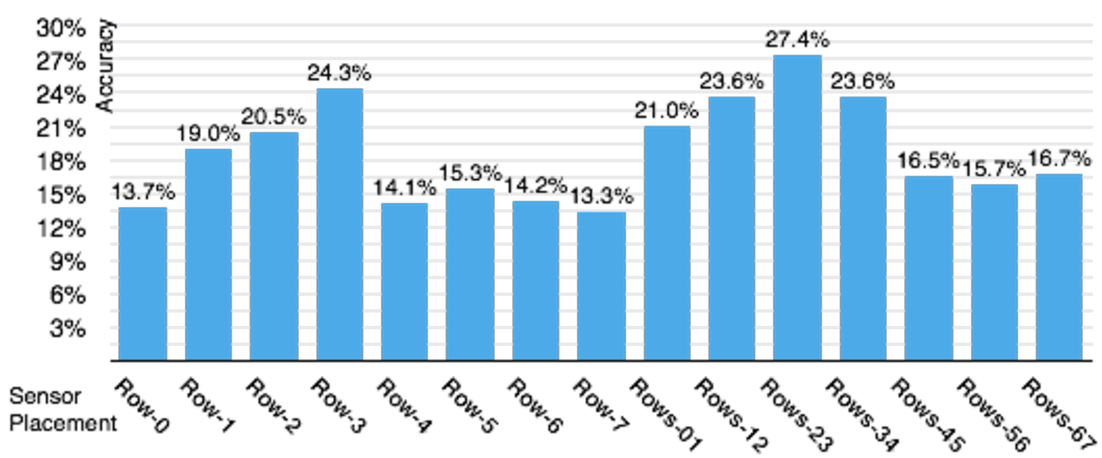
\includegraphics[width=1\columnwidth]{figures/LOO_V3.pdf}
  \caption{
    The result of the average of leave-one-user-out cross validations of all 10 participants.
    % The value of each bar is an average of test results of each participant at a location on the back of hand.
    The value of each bar is an average of test results of each participant validated by the other 9 participant's training model of a row configuration on the back of the hand.
  }
  \label{fig:LOO}
  \end{center}
\end{figure}

The results show that
(1) the configuration row-12 has the highest accuracy rate, indicating the most promising location is not on the closest row to the finger joints but second to it. 
(2) The accuracy rate of each single-row configuration is lower than that of its adjacent 2-row configuration. For example, the accuracy rate of configuration row-1 is lower than that of row-01 and row-12. Hence, the greater sensing resolution, the greater the accuracy rate is obtained. 
(3) The accuracy rates decrease along the rows as approaching to the wrist where physical signals become unrecognizable among hand gestures.

\section{DISCUSSION}

% Our discussion is divided into three subsections. 
% First of all, while most of the related work claimed support for small numbers of hand gestures (e.g. \(\leq 5\)), our prototype can support up to 16 hand gestures. We show all the classification rates for 16 gestures through confusion matrix for better insight into the differences and similarities among hand shapes.
% Secondly, the more gestures used, the lower the accuracy rates. We reduce the number of gestures to 5 in order to present its performance under a different scenario for small numbers of gestures.
% Thirdly,

Our discussion is divided into three subsections. 
First of all, we show all the classification rates for 16 gestures through confusion matrix for better insight into the differences and similarities among hand shapes.
Secondly, we reduce the number of gestures to 5 in order to present its performance under a different scenario for small numbers of gestures.
Thirdly, prototype limitations are listed to address some main factors for improvement.
\begin{figure}[h]
  \begin{center}
  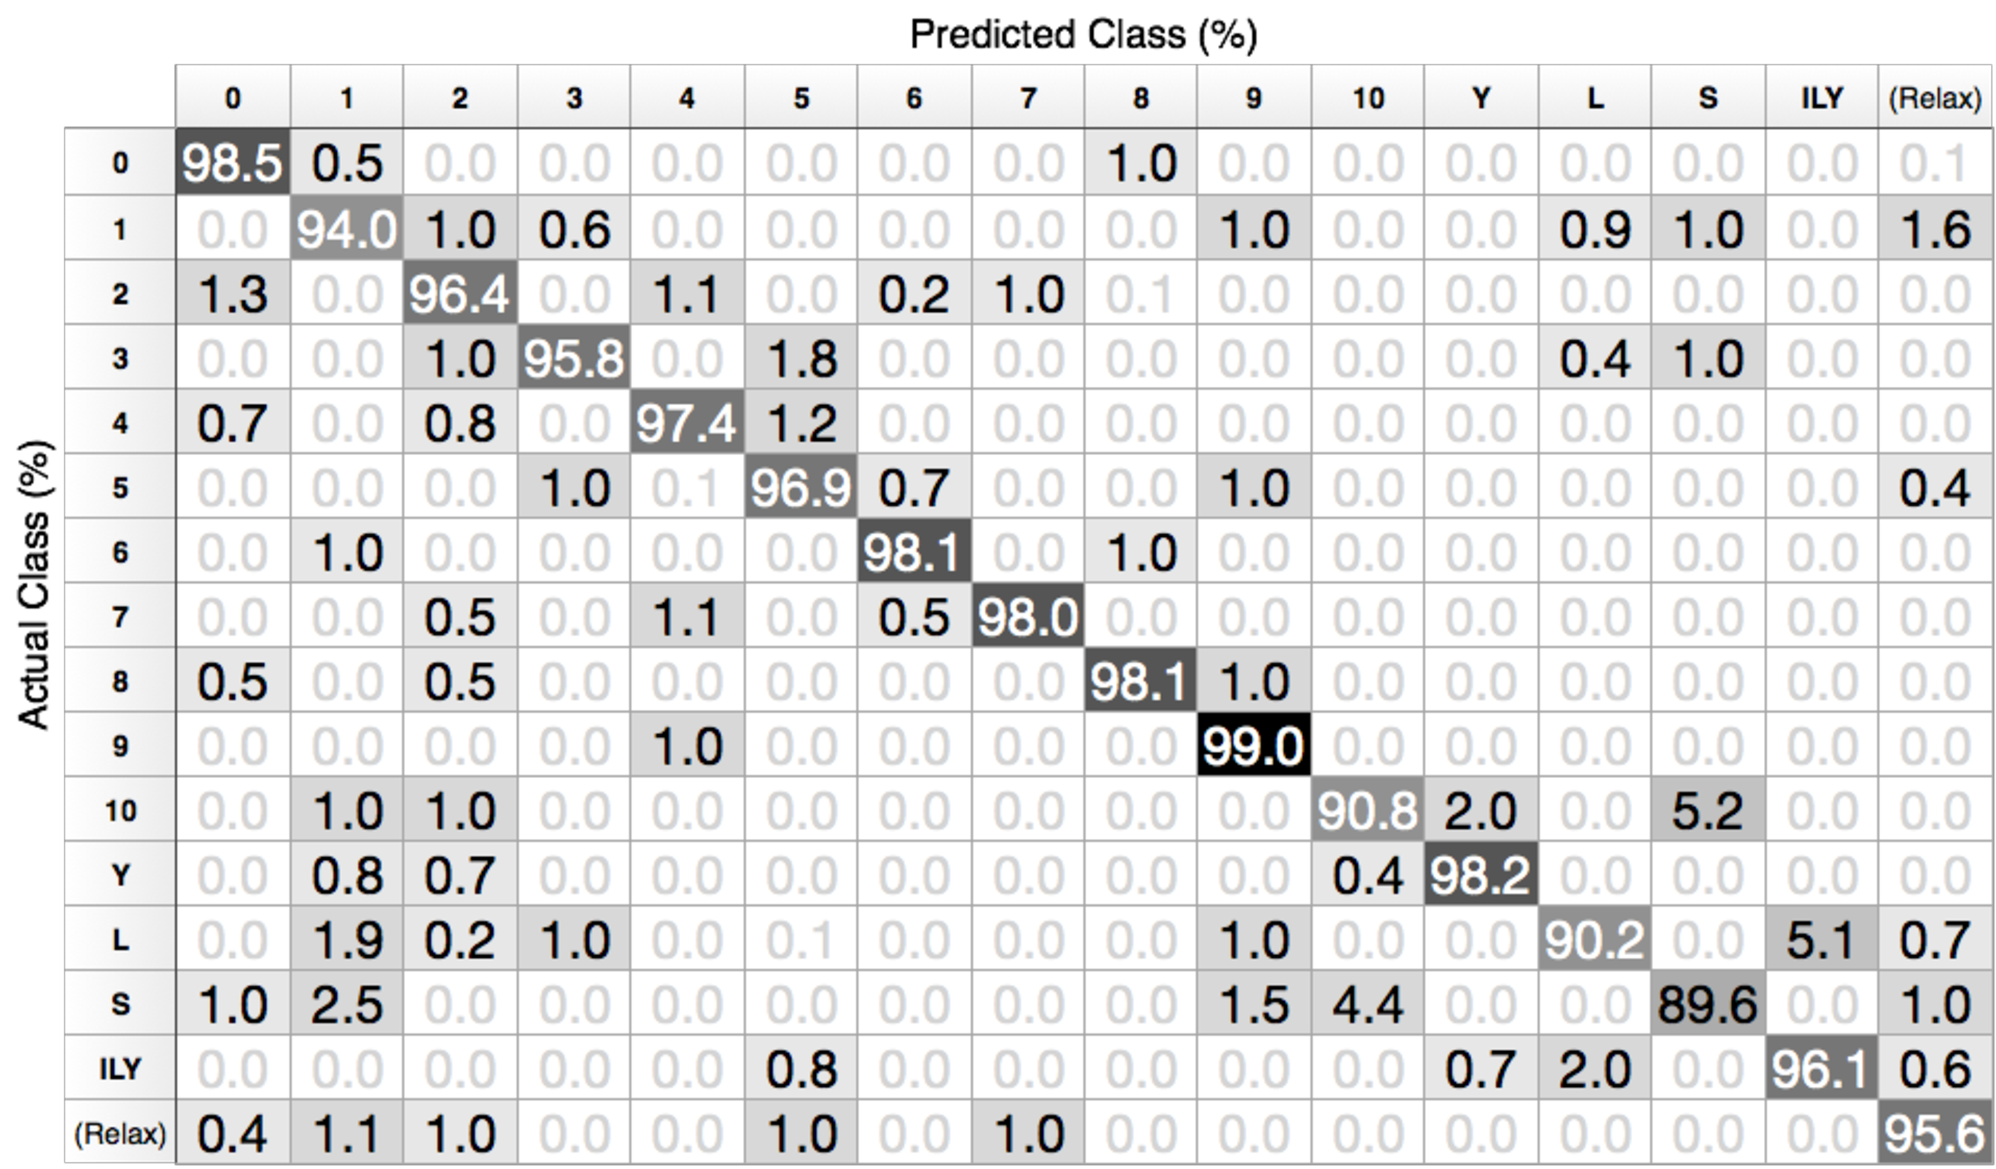
\includegraphics[width=1\columnwidth]{figures/CM_row12_v2.pdf}
  \caption{Confusion matrix for accuracies using training data from the row configuration of row12.}
  \label{fig:CM_row12}
  \end{center}
\end{figure}
\subsection{Confusion Matrix}

A confusion matrix shown in \autoref{fig:CM_row12}\ describes the misclassification rates of the gestures using the configuration row-12.
The occurrence of false detection is usually resulted from the similarities of handshapes.
For instance, the ``S'' gesture has the lowest true positive rate (89.6\%) among 16 gestures and has a chance of 4.4\% to be classified as the ``10'' gesture because the two gestures only differ by the thumb posture.
Another reason for misclassification is associated with weak physical signals.
For example, the ``L'' gesture has a true positive rate (90.2\%) and a false negative rate of 5.1\% for being classified as the ``ILY'' gesture likely because the  physical changes caused by movements of the pinky finger are less obvious compared to that of other fingers. Therefore, an increase in the amplifier gain leads to a better effectiveness in extracting weak signals.
% Overall, most of 16 gestures have a true positive rate greater than 90\% from which it is reasonable to infer that the back of hand is an excellent signal source for a gestural interface.
Overall, the true positive recognition rates are greater than 90\% for 15 gestures and 95\% for 12 gestures out of 16 gestures. From such result, it is reasonable to infer that the back of hand is an excellent signal source for a hand gesture interface.

\subsection{Signal Source Comparison}
To verify our assumption that the closer the signal source is to the fingers, the greater the accuracy rate of finer gesture recognition is obtained, a comparison is made with a related work \cite{Dementyev:2014:WLG:2642918.2647396} as in which we use the exact same setup except for the on-screen feedback. Currently, WristFlex \cite{Dementyev:2014:WLG:2642918.2647396} is a work with the highest accuracy rates (\textgreater80\%) supporting the ample number of gestures (5 gestures) among other works using wrist-based signal source.
% To verify our results that the closer the signal source is to the wrist, a significant decrease in accuracy rate of gesture recognition is obtained, a comparison is made with a related work, WristFlex, as in which we use the exact same setup except for an on-screen feedback.
We choose the 4 pinching gestures and a relaxed gesture \cite{Dementyev:2014:WLG:2642918.2647396} which are also included in our gesture set. We pick the training data from the most promising location. The methods to compute the accuracy rates are exactly the same as \cite{Dementyev:2014:WLG:2642918.2647396}. The accuracy rate obtained from the back of hand is statistically greater than that from the wrist in a 10-fold cross validation (98.2\% vs 96.3\%) and in a real-time cross validation with 3 training trials and 6 testing trials without feedback (90.6\% vs 69.3\%). The results indicate that sensing from the back of hand leads to a higher accuracy rate due to its close proximity to the fingers.

\subsection{Limitations}
Aforementioned in the leave-one-user-out cross validation, a small likelihood of a generalized model to fit all users is one of the limitations of utilizing such signal source.

Our prototype employs strain sensors which are meant to measure very small strain and elongation of a rigid structure. The sensors can be damaged by applying an excessive stress while removing the artificial skin off the user. High elongation strain gauges can be adopted to resolve this problem.

% artificial skin adhesion
Although we picked a highly reusable hydrogel-based artificial skin that can be used repeatedly across 10 participants in our user study, the artificial skin absorbs perspiration which decreases the adhesion for fixation on skin. We continue to look for alternative solutions such as "smart skin" systems that integrates this sensing technique with other modalities that warrant or even require to be located on the back of the hand.

The signals from the sensors must undergo stages of signal processing and conditioning leading to a number of chips required in the hardware taking up space in our prototype. Thus, the current size of our hardware is not suitable for an on-body hand gesture interface. Moreover, the system requires a USB serial cable for power supply and data transmission. It will be future work to redesign a small sized, battery powered, and wireless hardware.

%\vspace{10mm}
\begin{figure}[h]
  \begin{center}
  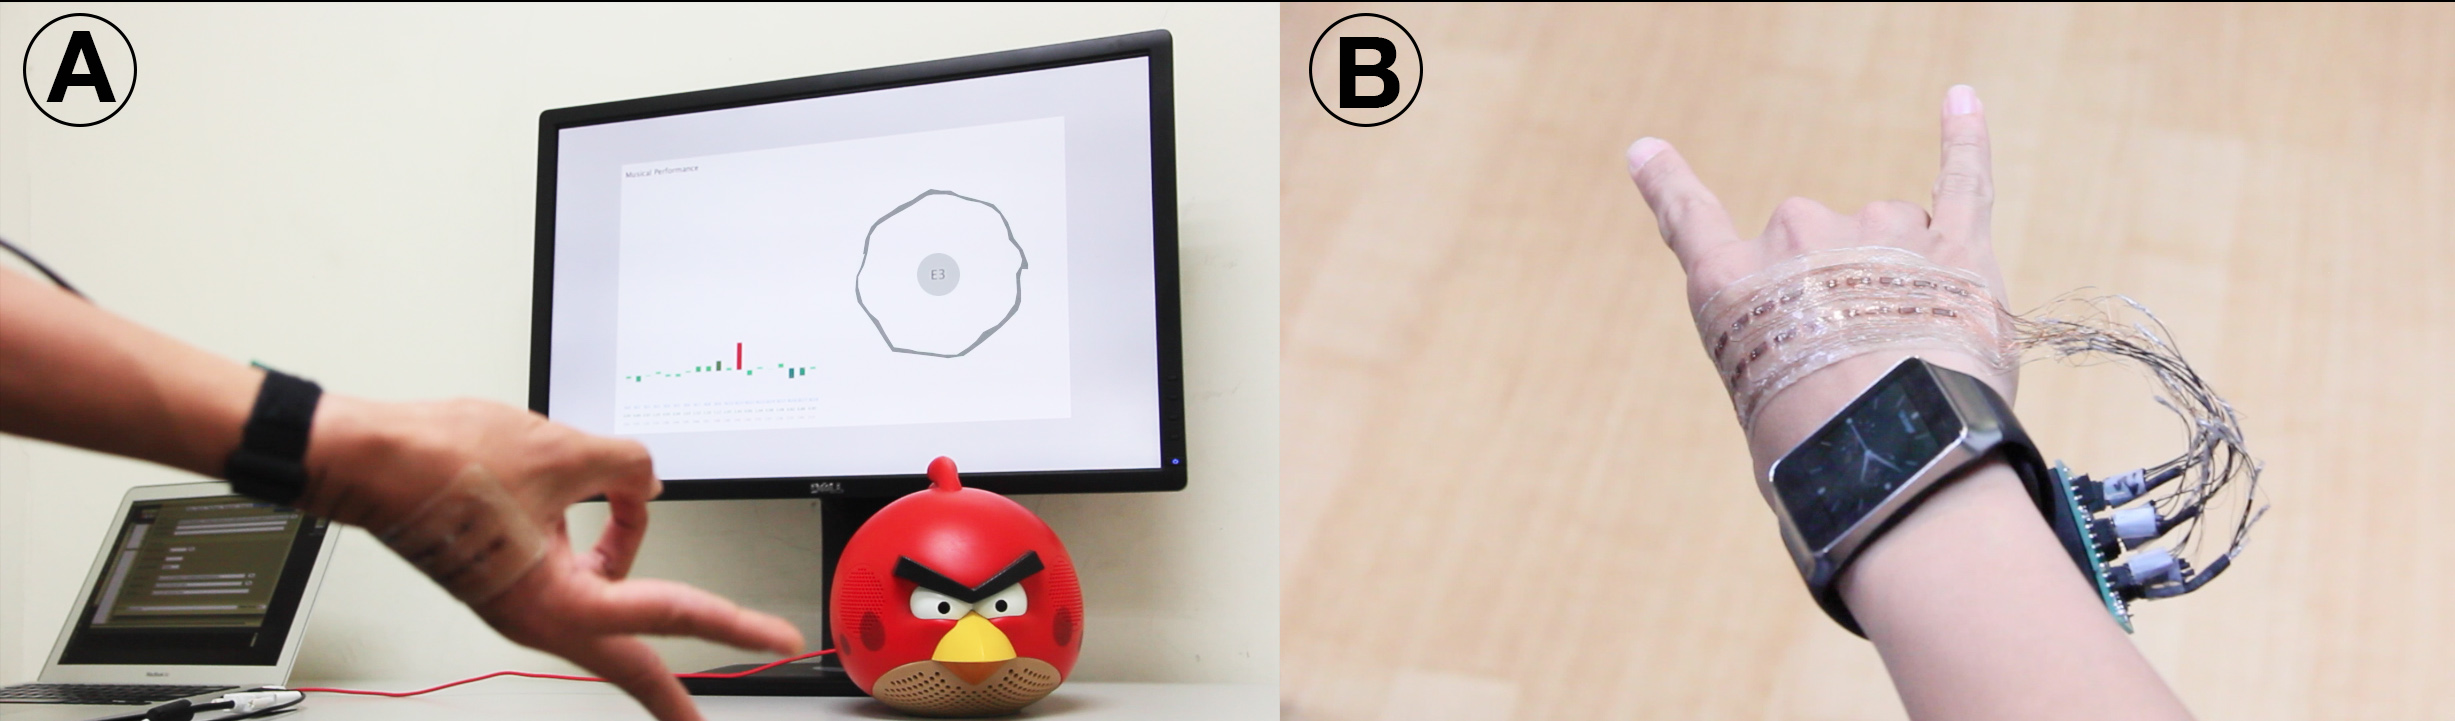
\includegraphics[width=1\columnwidth]{figures/appsV2.jpg}
  \caption{(A) A musical performance application turns the hand into a musical instrument. Gestures are translated into musical notes. (B) A smartwatch control provides a more user friendly, intuitive hand gesture interface.}
  \label{fig:APPS}
  \end{center}
\end{figure}

\section{EXAMPLE APPLICATIONS}

In additional to gesture recognition for general applications, we broadened the application of \getTitleName\ by showing a musical performance application and smartwatch control using static and dynamic gestures, respectively.
\vspace{10mm}
\subsection{Musical Performance}
% \getTitleName\ can distinguish the small difference among the hand gestures. We develop an application that hands become the musical instrument and the designated gestures will be translated to different musical notes. Tip segments of first, second, third,  little fingers and bottom segments of first, second, third fingers are Do, Re, Mi, Fa, Sol, La, Ti in C major respectively. By the system, hands are  wearable musical instrument and users can easily play them.

Since \getTitleName\ can distinguish finer gestures, we developed an application which turns the hand into a musical instrument whose musical notes are translated from designated gestures. The pinch gestures such as the ``9'', ``8'', ``7'', and ``6'' gestures from ASL are translated into musical notes of ``Do'', ``Re'', ``Mi'', and ``Fa'', respectively in C major. Similar to the pinch gestures, the thumb makes physical contact with the bottom segment of the index, middle, and ring finger to generate the rest of the musical notes of ``Sol'', ``La'', and ``Si'', respectively, in a C major scale. \getTitleName\ can be turned into a wearable musical instrument that can increase productivity and be entertaining.

\subsection{Smartwatch Control}
% Based on the high data rate and the diversity of gesture types of \getTitleName, finger movement can control smartwatch without the help of the other hand. Users are able to customize several input gestures. For example, the movement of thumb skip to the next page and the ``9'' gesture from ASL is selection. The application makes smartwatch control more convenient because users can simply make the input gesture without touching the so small screen. 

Due to the high data rate and a variety of gestures supported by \getTitleName, a smartwatch can be operated by a single hand. Users are able to customize the input gestures. For example, sliding the thumb across the index finger skips to the next page, and the ``9'' gesture from ASL makes a confirmation command. The application makes smartwatch control more user friendly by providing an intuitive gestural input and without the need for touching the small screen. 

    
% Use a numbered list of references at the end of the article, ordered
% alphabetically by first author, and referenced by numbers in
% brackets~\cite{ethics, Klemmer:2002:WSC:503376.503378,
%   Mather:2000:MUT, Zellweger:2001:FAO:504216.504224}. For papers from
% conference proceedings, include the title of the paper and an
% abbreviated name of the conference (e.g., for Interact 2003
% proceedings, use \textit{Proc. Interact 2003}). Do not include the
% location of the conference or the exact date; do include the page
% numbers if available. See the examples of citations at the end of this
% document. Within this template file, use the \texttt{References} style
% for the text of your citation.

% Your references should be published materials accessible to the
% public.  Internal technical reports may be cited only if they are
% easily accessible (i.e., you provide the address for obtaining the
% report within your citation) and may be obtained by any reader for a
% nominal fee.  Proprietary information may not be cited. Private
% communications should be acknowledged in the main text, not referenced
% (e.g., ``[Robertson, personal communication]'').

% \begin{table}
%   \centering
%   \begin{tabular}{r c c}
%     \toprule
%     & \multicolumn{2}{c}{\small{\textbf{Caption}}} \\
%     \cmidrule(r){2-3}
%     {\small\textbf{Objects}}
%     & {\small \textit{Pre-2002}}
%     & {\small \textit{Current}} \\
%     \midrule
%     Tables & Above & Below \\
%     Figures & Below & Below \\
%     \bottomrule
%   \end{tabular}
%   \caption{Table captions should be placed below the table. We
%     recommend table lines be 1 point, 25\% black. Minimize use of
%     unnecessary table lines.}~\label{tab:table1}
% \end{table}


\section{Conclusion}
We made a classification for hand gesture interfaces based on the three common input signal sources, each of which was briefly introduced with its principle and its several characteristics such as gestural recognition rate, computational overhead, finger dexterity, comfort, limitations, and so forth. Based on our classification, in general, the closer the source is to the fingers, the greater the accuracy rate of gestural recognition is obtained.
% We managed to combine the beneficial characteristics of previous works through a different approach by exploring the back of hand where it is used as a signal source.
The back of the hand is a new category of input signal source and is closer to fingers where obvious tendon movements are located. Sensing at this location causes less interference with finger agility. We implemented a prototype, \getTitleName, whose sensing stage consists of a reusable artificial skin and an array of 19 strain gauge sensors in a 2-row configuration which measure physical changes at multiple spots on the back of hand.

A user study was conducted to better understand gesture recognition accuracy and the effects of sensing locations. A set of 16 gestures was chosen from both American Sign Language and popular Asian gestures. We collected 8 rows of data from the participants' back of hand and employed SVM machine learning technique to discern 16 gestures. Our results showed that the most promising location spans from the second row to the third row starting off from the metacarpophalangeal joints. The highest leave-one-user-out average gestural recognition accuracy rate is 27.4\% which becomes one of the limitations due to the significant different patterns on the back of hand across participants. However, the personalized average gestural recognition accuracy rate using the data from the most promising location reaches 95.8\% in a 10-fold cross validation. A visualization shown as heat maps indicating sensor reading patterns facilitates our understanding towards such phenomenon. We showed two example applications to inspire people with its potential use.
Our results provide future developers an alternative choice for input sources of hand gesture interface. 

% A comparison with a wrist-based gestural interface was made, and the results provide future developers an alternative choice for the input source of gestural interface. Finally, we concluded with example applications.

% \section{Acknowledgments}
% We thank our advisor Prof. Mike Y. Chen and the faculty and staff of National Taiwan University. We also express our gratitude towards all those who have helped us in our work.

% Balancing columns in a ref list is a bit of a pain because you
% either use a hack like flushend or balance, or manually insert
% a column break.  http://www.tex.ac.uk/cgi-bin/texfaq2html?label=balance
% multicols doesn't work because we're already in two-column mode,
% and flushend isn't awesome, so I choose balance.  See this
% for more info: http://cs.brown.edu/system/software/latex/doc/balance.pdf
%
% Note that in a perfect world balance wants to be in the first
% column of the last page.
%
% If balance doesn't work for you, you can remove that and
% hard-code a column break into the bbl file right before you
% submit:
%
% http://stackoverflow.com/questions/2149854/how-to-manually-equalize-columns-
% in-an-ieee-paper-if-using-bibtex
%
% Or, just remove \balance and give up on balancing the last page.
%
\balance{}

% \section{References Format}


% REFERENCES FORMAT
% References must be the same font size as other body text.
\bibliographystyle{SIGCHI-Reference-Format}
\bibliography{sample}

\end{document}

%%% Local Variables:
%%% mode: latex
%%% TeX-master: t
%%% End:
